% Add the "twocolumn" argument to convert to 2 column format
% Add the "linenumbers" argument to include line numbers
% See this link for more info on how to use the documentclass
%  https://www.overleaf.com/project/6470f9cad6ea94bea26d41cb
\documentclass[]{aastex631}

\usepackage{BobsPreamble}

\newcommand*{\img}[1]{%
    \raisebox{-.3\baselineskip}{%
        \includegraphics[
        height=\baselineskip,
        width=\baselineskip,
        keepaspectratio,
        ]{#1}%
    }%
}

\begin{document}

\title{MHD Methods Paper}

\author[0000-0002-4475-3181]{Robert V. Caddy}
\affiliation{University of Pittsburgh, Department of Physics \& Astronomy \\
3941 O'Hara St \\ 
Pittsburgh, PA 15260, USA}

\author[0000-0001-9735-7484]{Evan E. Schneider}
\affiliation{University of Pittsburgh, Department of Physics \& Astronomy \\
3941 O'Hara St \\ 
Pittsburgh, PA 15260, USA}

\begin{abstract}

% S1: What are we presenting?
We present an extension of the massively parallel, GPU native, astrophysical hydrodynamics code Cholla to magnetohydrodynamics (MHD).
% S2: Which equations and methods?
Cholla solves the ideal MHD equations in their Eulerian form on a static Cartesian mesh utilizing the Van Leer + Constrained Transport integrator, the HLLD Riemann solver, and multiple reconstruction methods; including the piecewise parabolic method (PPM).
% S3: Performance results
Cholla's MHD module can perform over 150 million cell updates per GPU-second while using the HLLD Riemann solver and PPM.
% S4: How big of a grid can we do per GPU?
The massively parallel nature of GPUs allow Cholla's MHD module to perform simulation with resolutions of $>256^3$ cells on a single GPU.
% S5: Scaling
We use GPU direct MPI to attain nearly perfect weak scaling up to 74,000 GPUs and a total grid size of over 1.2 trillion cells.
% S6: We did test problems
A suite of test problems highlights the accuracy of Cholla's MHD module and demonstrate that it maintains zero magnetic divergence to round off error.
% S7: Summary of new testing framework
We also present the new testing and continuous integration tools for Cholla that utilize GoogleTest, GitHub Actions, and Jenkins.
% S8: Why Testing?
These new tools have allowed us to significantly increase our rate of development while making Cholla more robust and accurate.
% S9:  

\end{abstract}

% To Do for the plots
% - make plots that write out their info to a saved pickle dictionary
% - have a script to read in the proper link to the file
\section{asdf}
\input{|python ../python/get_links.py 'test_link' 'test text'}
for Constrained Transport (CT). CT treats the magnetic field as surface, rather than volume, averaged quantities then updates using edge averaged EMF (Electromotive Force). By updating with EMF you automatically fulfill the divergence free condition for magnetic fields so no magnetic monopoles will appear, assuming that the initial conditions are divergence free.
\href{http://www.overleaf.com}{\img{latex-src/orcid-ID.png}} 
for Constrained Transport (CT). CT treats the magnetic field as surface, rather than volume, averaged quantities then updates using edge averaged EMF (Electromotive Force). By updating with EMF you automatically fulfill the divergence free condition for magnetic fields so no magnetic monopoles will appear, assuming that the initial conditions are divergence free.

\section{Introduction}
\label{sec:intro}

% ==============================================================================
% Outline:
% - why do big sims matter?
%   - esp fast efficient MHD codes
%   - what kinds of sims?
%     - giant turbulent boxes, mhd outflows of galaxies
% - why this code? 
%   - why a new code? Cholla is fast, scales well, GPUs are fast, all big new 
%     computers are gpu based
%   - finite volume + CT, what other methods? Why is divergence cleaning bad
%   - cite lots of other codes and why is our code different
%   - why do we use this framework, what other options are there
%   - we have a testing framework that allows for scalable development, makes 
%     it easier and faster to dev since they don't have to worry about breaking 
%     other peoples stuff
% - Testing/CI stuff
% - outline paper
%   - alude to performance and testing at scale
% ==============================================================================

% - why do big sims matter?
%   - esp fast efficient MHD codes
Over the past decade it has become increasingly clear that magnetohydrodynamics (MHD) plays a significant role in a variety of astrophysical phenomena \citep[e.g.][]{shin_2008, beck_2016, banda_2016, naab_2017, han_2017, ntormousi_dynamo_2020, wibking_2021, gent_2021}. Magnetic fields couple to gas both directly through plasma interactions with the magnetic field, and indirectly through cosmic ray transport \citep[e.g.][]{pfrommer_simulating_2017, girichidis_spectrally_2019, chan_cosmic_2019, buck_effects_2020, werhahn_cosmic_2021, yoshida_trajectory_2021, girichidis_spectrally_2022, nunez-castineyra_cosmic-ray_2022, werhahn_gamma-ray_2023}, anisotropic conduction \citep[e.g.][]{yang_fermi_2012, hanasz_cosmic_2013, simpson_role_2016, girichidis_launching_2016, pakmor_galactic_2016, bruggen_2023}, and other physical effects.

% cite Arepo, Auriga, TNG, specific ones that I've talked about before

% I'd start this paragraph by bringing up the science problem, ideally linking it back to something you mentioned in the first paragraph of the introduction. Then you can explain why high resolution simulations are required to solve it.

% rephrase this less critically. I'd reframe the whole thing to suggest that these studies have provided intriguing hints of the possible effects of magnetic fields, but the results are not converged.
The role of magnetic fields in galactic structure is a matter of significant debate in the scientific literature. Different simulation methods, codes, and resolutions show varying impacts of magnetic fields, ranging from magnetic fields being largely irrelevant to large scale structure to magnetic fields being critically important in determining the evolution and structure of the interstellar medium (ISM), modifying galactic feedback, and the influencing the structure of the circumgalactic medium (CGM) \citep{banda_2016, pakmor_magnetic_2017, naab_2017, pakmor_faraday_2018, pakmor_magnetizing_2020, ntormousi_dynamo_2020, wibking_2021, van_de_voort_effect_2021}.

Many simulation projects, notably the Auriga Project \citep{grand_auriga_2017}, along with various followup analysis and simulations \citep{pakmor_faraday_2018,pakmor_simulations_2013,pakmor_magnetic_2017,pakmor_magnetizing_2020,ntormousi_dynamo_2020, hopkins_but_2020, van_de_voort_effect_2021} have attempted to determine the role of magnetic fields in galactic structure and have provided intriguing hints as to the possible effects of magnetic fields in galaxy dynamics. However, the lingering disagreements about the exact impacts of magnetic fields show that our understanding is not complete. A major reason for this uncertainty is the effect of numerical resolution in MHD simulations -- galactic magnetic fields are likely amplified by a turbulent dynamo which operates over a large dynamic range \citep{beck_1996, carteret_2022, brandenburg_2022}. Resolving this dynamo will require extremely high resolution MHD simulations -- simulations that are now possible thanks to recent developments in hardware, numerical algorithms, and software.

Modern numerical methods for MHD are sophisticated and robust, but even with highly optimized codes, MHD simulations remain very computationally expensive \citep{athena++_2020}. This computational expense is a result of the high number of floating point calculations required by modern finite-volume methods and the heavy memory bandwidth demands of MHD codes \citep{k_athena_2021}. In addition, MHD turbulent dynamos operate across a large dynamic range, from the full scale of a galaxy all the way down to a few parsecs or smaller, five or more orders of magnitude spatially \citep{ galishnikova_tearing_2022}. As a result, high resolution simulations are critical in order to accurately capture the effects of magnetic fields in astrophysical simulations. This need has driven a push to develop MHD codes that can take advantage of modern computer architectures \citep[e.g.][]{schive_gamer-2_2018, almgren_castro_2020, zingale_castro_2020, shankar_gram-x_2022, liska_h-amr_2022, begue_cuharm_2023, holmen_early_2023}. The computational expense of MHD simulations, along with the advent of Graphics Processing Units (GPUs) as the primary source of computational power in new cutting edge supercomputers\footnote{https://www.top500.org}, thus necessitates the development of GPU-based astrophysical MHD simulation codes. 

The induction equation requires that the magnetic field be divergence free, i.e. the Universe does not contain magnetic monopoles. However, not all numerical methods for evolving the MHD equations maintain this constraint. In many particle-based schemes, for example, magnetic divergence is generated and is removed at each step, a method commonly known as divergence cleaning \citep{dedner_hyperbolic_2002}. Divergence cleaning is popular because it couples well to particle-based methods -- it essentially functions by computing the divergence regularly and subtracting it away. Divergence cleaning is also computationally cheaper than numerical methods that maintain a divergence-free solution but typically leads to divergence errors on the level of a few percent \citep{dedner_hyperbolic_2002, pakmor_magnetizing_2020, van_de_voort_effect_2021}. While this error is small it could lead to unphysical solutions. However, a more accurate method for evolving the magnetic fields exists for grid based codes.

The other primary method for evolving the magnetic field in grid based codes is constrained transport (CT). Constrained transport is formally divergence free, and when implemented numerically it typically results in divergence errors on the order of machine round off error \citep{evans_1988, gardiner_2005, stone_athena_2008, stone_2009, zingale_castro_2020, almgren_castro_2020}. This is accomplished by tracking magnetic fields on a staggered, face centered grid rather than using cell-centered averages. These face centered values are used in conjunction with Riemann fluxes to calculate edge centered electric fields, and those electric fields are used to update the magnetic field. Thus, the trade-off for a divergence-free method is significant additional algorithmic complexity and associated computational expense.

% - why this code? 
%   - why a new code? Cholla is fast, scales well, GPUs are fast, all big new computers are gpu based
%   - finite volume + CT, what other methods? Why is divergence cleaning bad
%   - cite lots of other codes and why is our code different
%   - why do we use this framework, what other options are there
%   - we have a testing framework that allows for scalable development, makes it easier and faster to dev since they don't have to worry about breaking other peoples stuff
% Note that K-Athena is not related to Athena and is no longer under development, it does use CT. AthenaPK is under active development and uses divergence cleaning
The Cholla code (Computational Hydrodynamics On paraLLel Architectures) \citep{schneider_2015} is a fixed grid, finite volume hydrodynamics code for astrophysics that was designed to run natively on GPU-based supercomputers. It employs an unsplit 3D hydrodynamics integrator based on the Van Leer predictor-corrector method \citep{falle_1991, van_leer_2006} and was designed to be extended to MHD using constrained transport \citep{evans_1988, stone_athena_2008}. This work presents the MHD extension of Cholla. Our MHD implementation largely follows the Van Leer + Constrained Transport (VL+CT) method presented in \cite{stone_2009} with modifications for GPUs. It also uses an HLLD Riemann solver \citep{hlld_2005} and includes second \citep{stone_2009} and third \citep{felker_2018} order reconstruction in the characteristic variables \citep{stone_athena_2008}.

%   - what kinds of sims?
%     - giant turbulent boxes, mhd outflows of galaxies
The extension of Cholla to include MHD allows the simulation of previously unreachable domains. The VL+CT integrator provides high accuracy results with divergences that are zero to round off error. Given current memory constraints, the code is fast enough that a $\sim450^3$ cell MHD simulation can be run on a single high end GPU, allowing research-quality simulations to be run with only a small number of local resources. In addition, Cholla scales up to power of the largest available supercomputers, enabling simulations up to $19,278^3 \approx 7.2$ trillion cells on \textit{Frontier}\footnote{https://www.olcf.ornl.gov/frontier/}, the world's first exascale supercomputer. This will allow MHD simulations of entire galaxies with a constant resolution of a few parsecs per cell, turbulent box simulations with many trillions of cells, or many thousands of lower resolution simulations to be computed rapidly. For example, with approximately the same computing resources used to evolve a $19,278^3$ simulation one could run thousands of $2,000^3$-cell simulations, enabling entire parameter studies with resolutions comparable to current cutting edge CPU-based simulations.

% - Testing/CI stuff
In addition to requiring complex algorithms to produce accurate results, modern community-developed simulation codes like Cholla require robust testing and software-development infrastructure to maintain their reliability. This work also presents the implementation of an automated testing/continuous integration (CI) pipeline for Cholla. CI tools have expanded rapidly in functionality and popularity over the last 20 years and their usefulness in scientific software is well established \citep{beck_1999, wilson_2014,wilson_2017}. Particularly in the last 5 years with the advent of GitHub Actions and similar easily accessible and cheap (or even free) tools, CI pipelines have become much more straightforward to set up and run even for small groups and individuals. We present our implementation of testing and CI that is designed to be straightforward and scalable from a single GPU all the way up to an exascale machine. 

% - outline paper
%   - alude to performance and testing at scale
The outline of this paper is as follows. In Section \ref{sec:methods}, we describe our implementation of the VL+CT algorithm in detail along with the modifications we made to efficiently run on GPUs. In Section \ref{sec:mhd-tests}, we demonstrate the correctness and accuracy of Cholla on a suite of MHD test problems. We also describe Cholla's performance and weak scaling behavior on up to 74,088 GPUs using \textit{Frontier}. In Section \ref{sec:testing}, we discuss the new continuous integration and automated testing framework. We conclude in Section \ref{sec:summary}. In figure captions the GitHub icon, \img{../assets/github.png}, links to the version of the python script which generated that figure. These scripts, and the associated GitHub repository, have sufficient information to reproduce the figures shown in this paper.

% - [x] disclaimer, this is not new and based on all these sources. We order it slightly differently to work on GPUs so we will outline it here
% - [x] provide summary of integrator first then provide details. Then there's space in the first section to discuss details of the implementation
%  - [ ] How was this implemented on GPUs and what made it different
%    - [ ] what does Cholla do when I press go?
%      - [ ] allocations, data movement, etc
%  - [x] here's the details on all the math

\section{Methods}
\label{sec:methods}

Magnetic fields play a key role in many astrophysical phenomena, but are often neglected in numerical simulations due to the computational expense of magnetohydrodynamics. Part of this expense arises due to the wide range of temporal and physical scales over which magnetic field dynamos operate. Numerical integration of the MHD equations is also challenging; the additional waves compared to hydrodynamics and the requirement to maintain the divergence free condition result in considerable added complexity.

Given these considerations, MHD simulations often need to be both high resolution and use robust, divergence free methods, which tend to increase their computational cost. This limitation can be overcome by harnessing new GPU based supercomputers efficiently. Thus, we have elected to expand the existing massively parallel GPU-based hydrodynamics code, Cholla, to incorporate the effects of MHD. In this section we describe the equations solved and methods used by the MHD module of Cholla. While the algorithms themselves are not new, our particular combination of equations is not contained in any one reference, so we outline the full method here. We also highlight implementation choices that are particularly relevant to solving these equations on GPUs.

\subsection{Magnetohydrodynamics}
\label{sec:methods-mhd}

Cholla solves the ideal MHD equations in their conserved Eulerian form using a finite volume method \citep{Godunov}. These equations neglect all dissipative processes, including finite viscosity, electrical resistivity, and thermal conductivity. These approximations are reasonable when simulating regions of low density such as the ISM, CGM, and IGM. We note that although we neglect these additional processes at present, the methods implemented here are fully compatible with future extensions to include additional physics that depends on magnetic fields, such as anisotropic conduction, cosmic ray transport, or non-ideal MHD effects.

The ideal MHD equations are:

\begin{equation}
    \label{eqn:mass-conservation}
    \frac{\partial \rho}{\partial t} + \nabla \cdot (\rho \boldsymbol{v}) = 0
\end{equation}

\begin{equation}
    \label{eqn:momentum-conservation}
    \frac{\partial \rho\boldsymbol{v}}{\partial t} + \nabla \cdot (\rho \boldsymbol{v}\otimes\boldsymbol{v} - \boldsymbol{B}\otimes\boldsymbol{B} + P_T\boldsymbol{I}) = 0
\end{equation}

\begin{equation}
    \label{eqn:energy-conservation}
    \frac{\partial E}{\partial t} + \nabla \cdot ( (E + P_T) \boldsymbol{v} + \boldsymbol{B}(\boldsymbol{B}\cdot\boldsymbol{v}) ) = 0
\end{equation}

\begin{equation}
    \label{eqn:induction}
    \frac{\partial \boldsymbol{B}}{\partial t} - \nabla \times (\boldsymbol{v} \times \boldsymbol{B}) = 0
\end{equation}

\noindent where $\rho$ is density, $\boldsymbol{v} = ( v_x, v_y, v_z)$ is the velocity vector, $t$ is time, $\boldsymbol{B} = ( B_x, B_y, B_z)$ is the magnetic field, $\boldsymbol{I}$ is the identity tensor, $P_T \equiv P + \frac{1}{2}(\boldsymbol{B} \cdot \boldsymbol{B})$ is the total pressure, and $E$ is the total energy per unit volume $E \equiv \epsilon + \frac{1}{2}\rho(\boldsymbol{v}\cdot\boldsymbol{v}) + \frac{1}{2}(\boldsymbol{B}\cdot\boldsymbol{B})$. We adopt units in which the magnetic permeability $\mu_0 = 1$.

Equation \ref{eqn:mass-conservation} describes the conservation of mass, equation \ref{eqn:momentum-conservation} describes the conservation of momentum, equation \ref{eqn:energy-conservation} describes the conservation of energy, and equation \ref{eqn:induction} is the induction equation, which describes the divergence free condition. Cholla uses an ideal gas equation of state  which is $P \equiv \epsilon(\gamma - 1)$ where $\gamma$ is the adiabatic index and $\epsilon$ is the internal energy density.

In practice these equations are used in their vector form, where $\boldsymbol{U}$ and $\boldsymbol{W}$ are the conserved and primitive variables respectively:

\begin{align}
    \boldsymbol{U} &= \begin{bmatrix}
            \rho &
            v_x &
            v_y &
            v_z &
            E   &
            B_x &
            B_y &
            B_z
         \end{bmatrix}
    \\
    \boldsymbol{W} &= \begin{bmatrix}
            \rho &
            v_x &
            v_y &
            v_z &
            P   &
            B_x &
            B_y &
            B_z
         \end{bmatrix}.
\end{align}
The conservation equations, in Cartesian coordinates, can then be rewritten as

\begin{equation}
    \label{eqn:vector-conserved}
    \frac{\partial \boldsymbol{U}}{\partial t} +
    \frac{\partial \boldsymbol{F_x}}{\partial x} +
    \frac{\partial \boldsymbol{F_y}}{\partial y} +
    \frac{\partial \boldsymbol{F_z}}{\partial z} = 0
\end{equation}
where $\boldsymbol{F_x}$, $\boldsymbol{F_y}$, and $\boldsymbol{F_z}$ are the vectors of fluxes in the $x$, $y$, and $z$ direction respectively and are given by

\begin{equation}
    \boldsymbol{F_x} = \begin{bmatrix}
            \rho v_{x} \\
            \rho v_{x}^2 + P_{T} - B_{x}^2 \\
            \rho v_{x} v_{y} - B_{x} B_{y} \\
            \rho v_{x} v_{z} - B_{x} B_{z} \\
            v_{x} \left( E + p_{T} \right) - B_{x} \left( \boldsymbol{v} \cdot \boldsymbol{B} \right) \\
            0 \\
            B_{y} v_{x} - B_{x} v_{y} \\
            B_{z} v_{x} - B_{x} v_{z} \\
         \end{bmatrix}
\end{equation}

\begin{equation}
    \boldsymbol{F_y} = \begin{bmatrix}
            \rho v_{y} \\
            \rho v_{y} v_{x} - B_{y} B_{x} \\
            \rho v_{y}^2 + P_{T} - B_{y}^2 \\
            \rho v_{y} v_{z} - B_{y} B_{z} \\
            v_{y} \left( E + P_{T} \right) - B_{y} \left( \boldsymbol{v} \cdot \boldsymbol{B} \right) \\
            B_{x} v_{y} - B_{y} v_{x} \\
            0 \\
            B_{z} v_{y} - B_{y} v_{z} \\
         \end{bmatrix}
\end{equation}

\begin{equation}
    \boldsymbol{F_z} = \begin{bmatrix}
            \rho v_{z} \\
            \rho v_{z} v_{x} - B_{z} B_{x} \\
            \rho v_{z} v_{y} - B_{z} B_{y} \\
            \rho v_{z}^2 + P_{T} - B_{z}^2 \\
            v_{z} \left( E + P_{T} \right) - B_{z} \left( \boldsymbol{v} \cdot \boldsymbol{B} \right) \\
            B_{x} v_{z} - B_{z} v_{x} \\
            B_{y} v_{z} - B_{z} v_{y} \\
            0
         \end{bmatrix}.
\end{equation}


\subsection{The VL+CT Integrator}
\label{sec:vlct-summary}

To integrate these equations in Cholla, we implement the VL+CT (Van Leer plus Constrained Transport) integrator introduced in \cite{stone_2009}, along with the HLLD Riemann solver described in \cite{hlld_2005}. Many of the equations were first described in the context of the constrained-transport extension to the corner-transport upwind (CTU) method \citep{colella_1990} described in 2D \citep{gardiner_2005} and 3D \citep{gardiner_unsplit_2008} for the Athena MHD code \citep{stone_athena_2008}. Our specific implementation of the piecewise parabolic method follows \cite{felker_2018}, which is itself an extension of the original PPM method presented by \cite{colella_1984}. The VL+CT integrator is very similar in structure to the MUSCL-Hancock integrator \citep{van_leer_2006, falle_1991, Toro}, though with significant new additions for Constrained Transport (CT). We note that this is now the default integrator used in Cholla, as we have found it to be more robust than the CTU algorithm described in \cite{schneider_2015}.

Constrained transport treats the magnetic field as a surface averaged quantity centered at cell interfaces rather than a volume averaged, cell centered quantity like the hydro variables; i.e. a staggered grid. Each face stores only the magnetic field perpendicular to that face, i.e. the $x,i+1/2,j,k$ face stores the $B_{x,i+1/2,j,k}$ magnetic field. At each time step, the magnetic field is then updated using edge averaged electric fields computed from the magnetic flux returned by the Riemann solver. Updating the magnetic field with the electric field automatically fulfills the divergence free condition for magnetic fields, assuming that the initial conditions are also divergence free.

A brief overview of the algorithm for a single time step using the VL+CT integrator is as follows; more detailed discussion of each step is presented in the following subsections.

\begin{enumerate}
    \item Compute the time step, $\Delta t$.
    \item Reconstruct interface states using a piecewise constant method (PCM) approximation.
    \item Solve the Riemann problem on every interface using the PCM interface states.
    \item Compute the edge centered electric fields.
    \item Update the $t=n$ conserved variables to $t=n+\Delta t/2$ using the computed fluxes and electric fields.
    \item Reconstruct interface states using a piecewise linear method (PLM) or piecewise parabolic method (PPM) approximation.
    \item Solve the Riemann problem on every interface using the higher order reconstructed interface states.
    \item Recompute the edge centered electric fields.
    \item Update the $t=n$ conserved variables to $t=n+\Delta t$ using the half time step fluxes and electric fields
\end{enumerate}

% ===========================================================================

\subsubsection{Step 1: Compute the Time Step}
\label{vlct:dt}

The first step is to compute the time step. Cholla implements uniform time steps across the grid, so this is the minimum crossing time of any wave in any cell multiplied by a Courant factor to maintain the Courant–Friedrichs–Lewy condition \cite{cfl}:

\begin{equation}
        \label{eqn:dt}
        \Delta t = C_{CFL} \min \left(
            \frac{\Delta x}{\mid v^n_{x,i,j,k} \mid + c^n_{f,i,j,k}},
            \frac{\Delta y}{\mid v^n_{y,i,j,k} \mid + c^n_{f,i,j,k}},
            \frac{\Delta z}{\mid v^n_{z,i,j,k} \mid + c^n_{f,i,j,k}}
        \right),
\end{equation}

\noindent where $\Delta t$ is the time step, $C_{CFL} \leq 0.5$ is the CFL number, $\mid v^n_{l,i,j,k}\mid $ is the magnitude of the velocity in the $l$ direction velocity in the ${i,j,k}$ cell, and $c^n_f $ is the fast magnetosonic wave-speed computed using \emph{cell centered} values. The fast and slow magnetosonic speeds are

\begin{equation}
    c_{f,s} = \sqrt{\frac
    {\gamma p + \mid \boldsymbol{B} \mid^2 \pm \sqrt{\left( \gamma p \;+ \mid \boldsymbol{B} \mid^2 \right)^2 - 4\gamma p B_x^2 } }
    {2\rho}}
\end{equation}

\noindent where the $+$ option corresponds to the fast magnetosonic speed, and $-$ to the slow.

Equation \ref{eqn:dt} computes the minimum crossing time of a wave in a specific cell. A global reduction is then performed to find the minimum in the entire grid; that minimum is used as the time step $\Delta t$. This reduction is done primarily on the GPU followed by an MPI ALL\_REDUCE. Because GPUs programming methods are inherently parallel, GPU reductions are not trivial and their performance is sensitive to the method used. Details of our reduction method are discussed in section \ref{sec:gpu-vs-cpu}.

The cell-centered magnetic field is computed with a direct average of the face centered values:
\begin{equation}
    \begin{aligned}
        B^n_{x,i,j,k,} = \frac{1}{2} \left( B^n_{x,i+1/2,j,k} + B^n_{x,i-1/2,j,k} \right) \\
        B^n_{y,i,j,k,} = \frac{1}{2} \left( B^n_{y,i,j+1/2,k} + B^n_{y,i,j-1/2,k} \right) \\
        B^n_{z,i,j,k,} = \frac{1}{2} \left( B^n_{z,i,j,k+1/2} + B^n_{z,i,j,k-1/2} \right) \\
    \end{aligned}
\end{equation}
These cell-centered values for the magnetic field are used several times throughout the integrator. In CPU-based codes it is typically more efficient to compute these cell centered magnetic fields once and save them, since traditional CPU-based codes are typically compute limited. Cholla is generally limited instead by GPU memory, so we recompute the cell-centered values when they are needed rather than permanently allocating the associated memory.



\subsubsection{Step 2: First Order Reconstruction}
\label{vlct:first-order-reconstruction}

Reconstructing the interface states at first order, or the piecewise constant method (PCM), is done by setting the primitive interface states values to the same value as the cell:

\begin{equation}
    \boldsymbol{W}_{L, i+1/2} = \boldsymbol{W}_{R, i-1/2} = \boldsymbol{W}_{i}
\end{equation}

\noindent where $ \boldsymbol{W}_{L/R, i\pm1/2} $ is the state on the left or right side of the cell. Although Cholla evolves the conserved variables, primitive variables are typically used for interface reconstruction since they are required by the Riemann solver used to compute the fluxes. In higher order spatial reconstructions we also use the characteristic variables derived from the primitive variables.

Although PCM is too diffusive to be used on its own in both reconstruction steps, we note that that mode is excellent for debugging. Here, it offers a computationally-inexpensive way to calculate first-order fluxes, which will be used for the ``predictor" step of this predictor-corrector algorithm. Most higher order methods revert to PCM near large discontinuities.

\subsubsection{Step 3: First Riemann Solve}
\label{vlct:first-riemann-solve}

The next step is to solve the Riemann problem with the first order interface states. To do this, we employ the HLLD Riemann solver introduced in \cite{hlld_2005}. Because we have implemented the Riemann solver exactly as described in \cite{hlld_2005} we do not reproduce all the details here. The longitudinal magnetic field does not require reconstruction and can be used directly since it is stored at the face. The transverse fields (i.e. the fields parallel to the interface) are reconstructed from the cell centered average (computed as shown in section \ref{vlct:dt}), then reconstructed using PCM identically to other fields.

The magnetic fluxes returned by the Riemann solver are the face centered electric fields \citep[see section 5.3 of][]{stone_athena_2008}. For clarity, we list in Table \ref{table:emf} the correlation between flux and electric field.

\begin{deluxetable*}{llll}
    \label{table:emf}
    \tablecaption{Magnetic Flux to Face Centered electric field}

    \tablehead{\colhead{HLLD Solve Direction} & \colhead{Equation for Magnetic Flux} & \colhead{Eqn. as a Cross Product} & \colhead{electric field}}

    \startdata
    $ X $ & $ V_x B_y - B_x V_y $ & $  (V \times B)_z $ & $ -\varepsilon_z $ \\ \hline
    $ X $ & $ V_x B_z - B_x V_z $ & $ -(V \times B)_y $ & $  \varepsilon_y $ \\ \hline
    $ Y $ & $ V_x B_y - B_x V_y $ & $  (V \times B)_z $ & $ -\varepsilon_x $ \\ \hline
    $ Y $ & $ V_x B_z - B_x V_z $ & $ -(V \times B)_y $ & $  \varepsilon_z $ \\ \hline
    $ Z $ & $ V_x B_y - B_x V_y $ & $  (V \times B)_z $ & $ -\varepsilon_y $ \\ \hline
    $ Z $ & $ V_x B_z - B_x V_z $ & $ -(V \times B)_y $ & $  \varepsilon_x $ \\ \hline
    \enddata

    \tablecomments{The directions used here are relative to the internal workings of the HLLD solver. Since the HLLD solver is inherently 1D we run it once for each of the faces of a cell. So in the case where the solver is running in the Y direction the solver's Y field is actually the Z field and the solver's Z field is actually the X field, cyclically extended for the Z direction.}
\end{deluxetable*}

\subsubsection{Step 4: Compute the Constrained Transport Electric Field}
\label{vlct:emf}

The next step is to calculate the constrained transport electric field. These fields are \emph{line averaged} along each cell vertex. These line averaged fields are constructed by averaging the face centered electric fields from the previous step, and their slopes. Equation \ref{eqn:emf-edge} is used to reconstruct these line averaged electric fields; only the equation for the $ z $-direction is presented, the equations for the other directions can be found by cyclic permutation. The equations for computing the other directions are obtained by substituting out the $ z $ index with $ x $ or $ y $ and changing the derivatives appropriately.

\begin{equation}
    \label{eqn:emf-edge}
    \begin{aligned}
        \mathcal{E}_{z, i-1/2, j-1/2, k} = \frac{1}{4} \left(
              \mathcal{E}_{z, i-1/2, j, k}
            + \mathcal{E}_{z, i, j-1/2, k}
            + \mathcal{E}_{z, i-1/2, j-1, k}
            + \mathcal{E}_{z, i-1, j-1/2, k}\right) \\
        + \frac{\Delta y}{8} \left( \left( \frac{\partial \mathcal{E}_z }{\partial y} \right)_{i-1/2, j-1/4, k} + \left(  \frac{\partial \mathcal{E}_z }{\partial y} \right)_{i-1/2, j-3/4, k} \right) \\
        + \frac{\Delta x}{8} \left( \left( \frac{\partial \mathcal{E}_z }{\partial x} \right)_{i-1/4, j-1/2, k} + \left(  \frac{\partial \mathcal{E}_z }{\partial x} \right)_{i-3/4, j-1/2, k} \right)
    \end{aligned}
\end{equation}

$\mathcal{E}_{z, i-1/2, j-1/2, k}$ is the line averaged electric field; the first four terms on the right are the face averaged electric fields, and the four derivative terms are the derivatives of those fields in the direction towards the edge, details of which are in Equation \ref{eqn:emf-slope}. Figure \ref{fig:emf-graph} shows the spatial relationships between the derivatives and the relevant edge states and reference fields. Each edge requires 4 derivatives and they are computed as differences between a reference state and an edge state.

Technically, constrained transport uses the magnetic flux as the conserved variable and EMF (ElectroMotive Force) to update it. However, because those values only differ from the magnetic flux density (i.e. the magnetic field) and the electric field respectively by factors of unit length either can be treated as the conserved variable, the same way either density or mass can be evolved in the hydro fields \citep{stone_athena_2008}. As such we use the magnetic field and electric field to evolve the grid. Electric fields have the proper units to evolve the magnetic flux density, $ B $, whereas EMF has the proper units to evolve the magnetic flux.

On any face there are two non-zero electric fields; both transverse to the face. The component that is used to calculate the field along a given edge is the component that is parallel to that edge; i.e. if the edge points along the $ z $-direction then the field pointing along the $ z $-direction is used, not the field in the $ x $ or $ y $ direction.

The derivatives from Equation \ref{eqn:emf-edge} are computed using the upwinded slope as follows

\begin{equation}
    \label{eqn:emf-upwind-slope}
    \left( \frac{\partial \mathcal{E}_z }{\partial y} \right)_{i-1/2, j-1/4, k} =
        \begin{cases}
            \left( \frac{\partial \mathcal{E}_z }{\partial y} \right)_{i-1, j-1/4, k} & \text{for} \; v_{x, i-1/2} > 0
            \\
            \\
            \left( \frac{\partial \mathcal{E}_z }{\partial y} \right)_{i, j-1/4, k} & \text{for} \; v_{x, i-1/2} < 0
            \\
            \\
            \frac{1}{2} \left( \left( \frac{\partial \mathcal{E}_z }{\partial y} \right)_{i-1, j-1/4, k} + \left( \frac{\partial \mathcal{E}_z }{\partial y} \right)_{i, j-1/4, k} \right) & \text{otherwise}
            \\
            \\
        \end{cases}
\end{equation}

\noindent where, for example, the derivatives are given by

\begin{equation}
    \label{eqn:emf-slope}
    \left( \frac{\partial \mathcal{E}_z }{\partial y} \right)_{i, j-1/4, k} =
    2 \left( \frac{\mathcal{E}_{z,i,j-1/2,k} - \mathcal{E}_{z,i,j,k}^{ref}}{\Delta y} \right).
\end{equation}

\noindent $\mathcal{E}_{z,i,j,k}^{ref}$, is the cell centered reference field. This reference field is computed with the following cross product

\begin{equation}
    \mathcal{E}_{i,j,k}^{ref,n} = - \left( \boldsymbol{v}^{n}_{i.j.k} \times \boldsymbol{B}^{n}_{i.j.k} \right).
\end{equation}

\begin{figure}[ht!]
    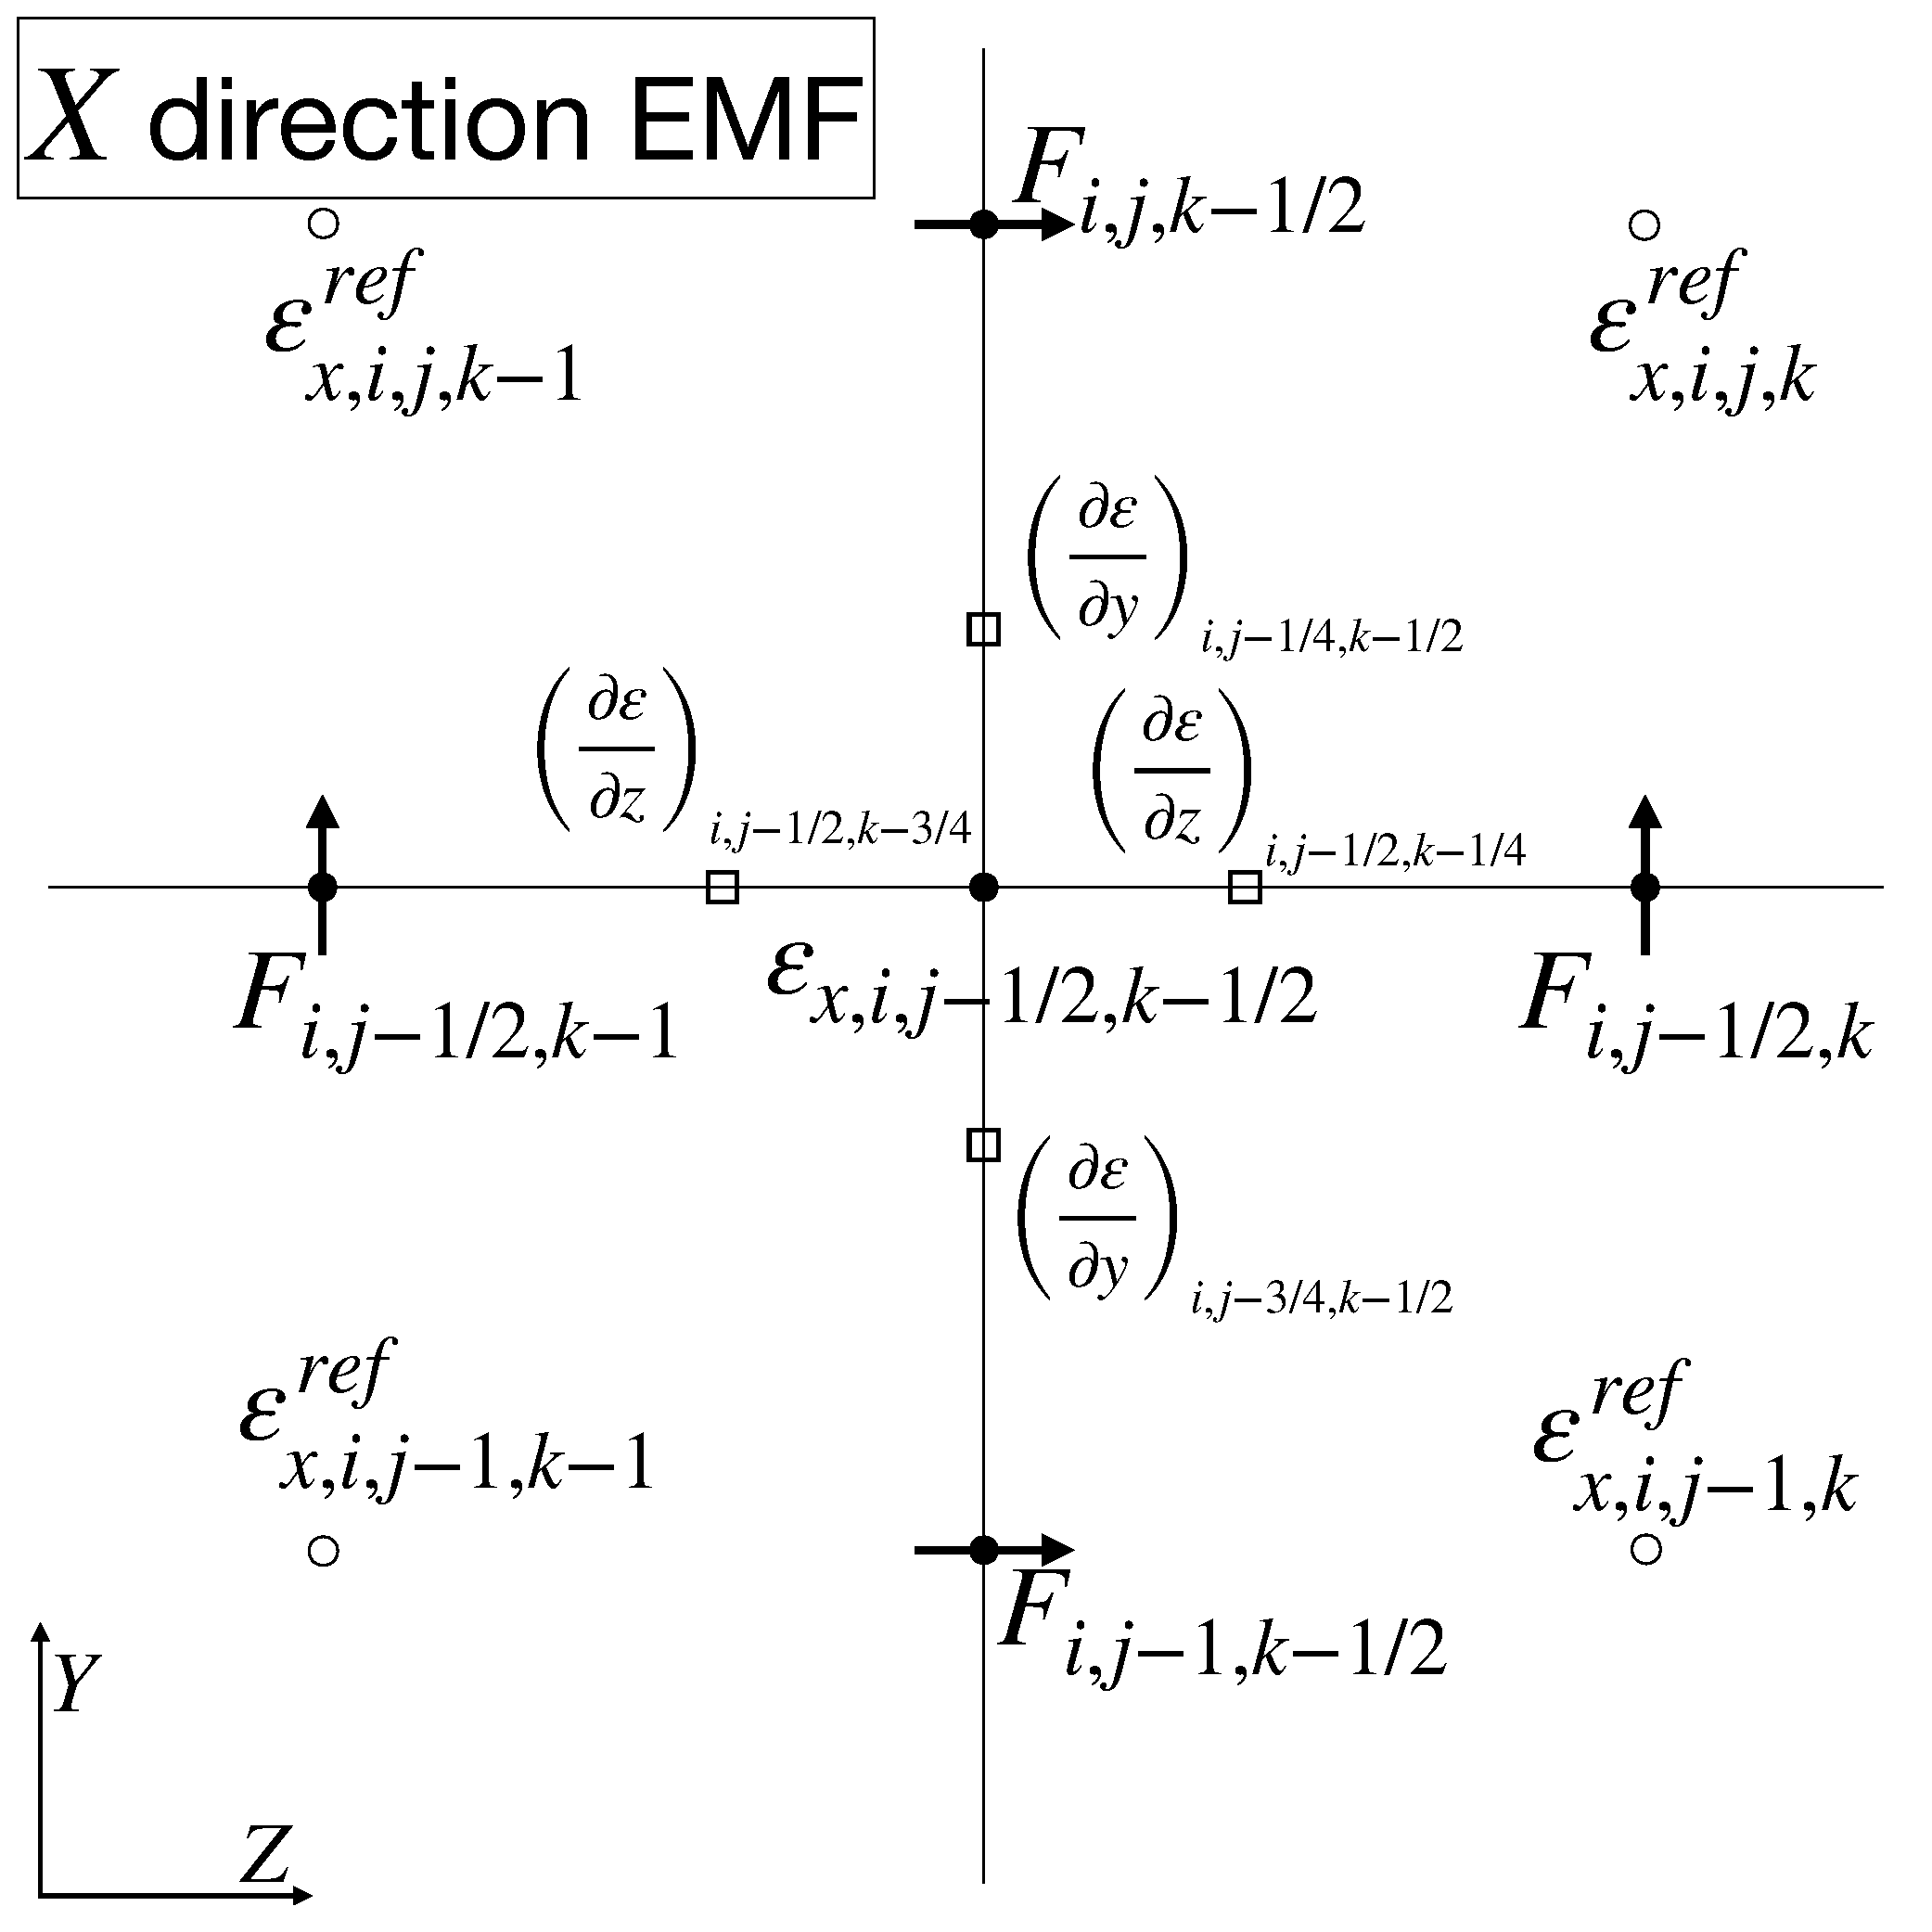
\includegraphics[width=0.5\linewidth]{CT-edge-field-figures-X.pdf}
    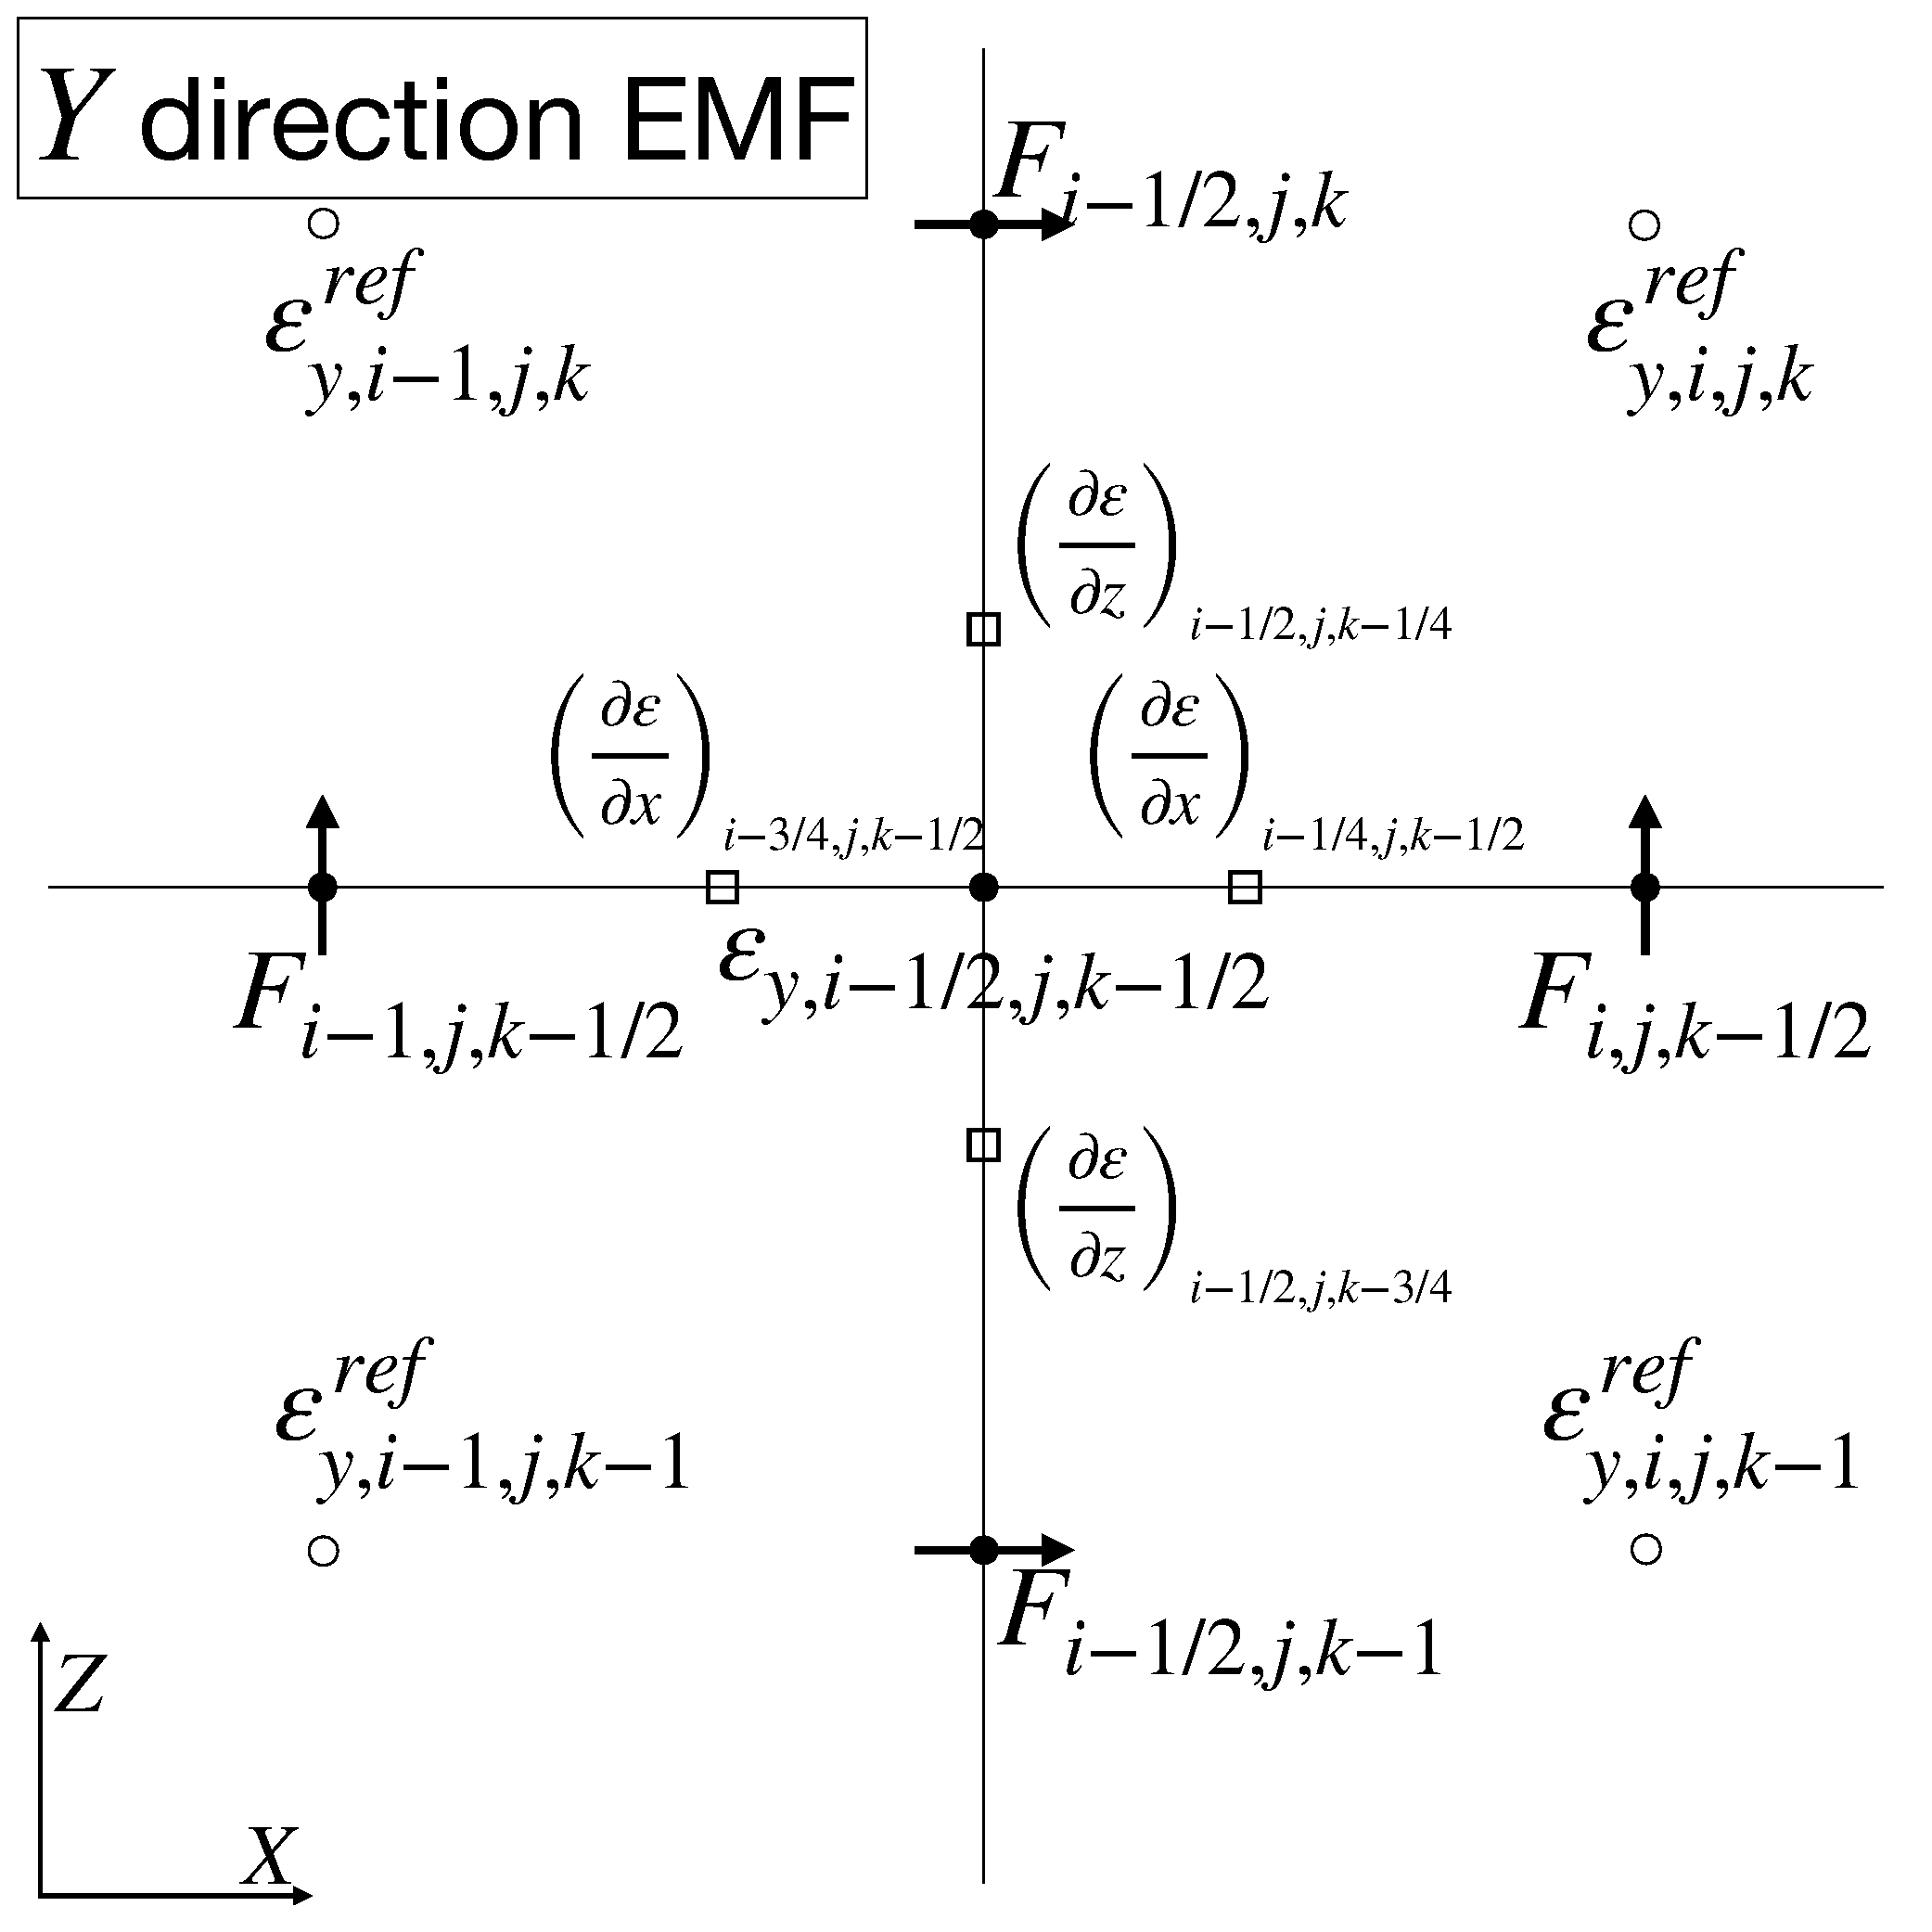
\includegraphics[width=0.5\linewidth]{CT-edge-field-figures-Y.pdf}
    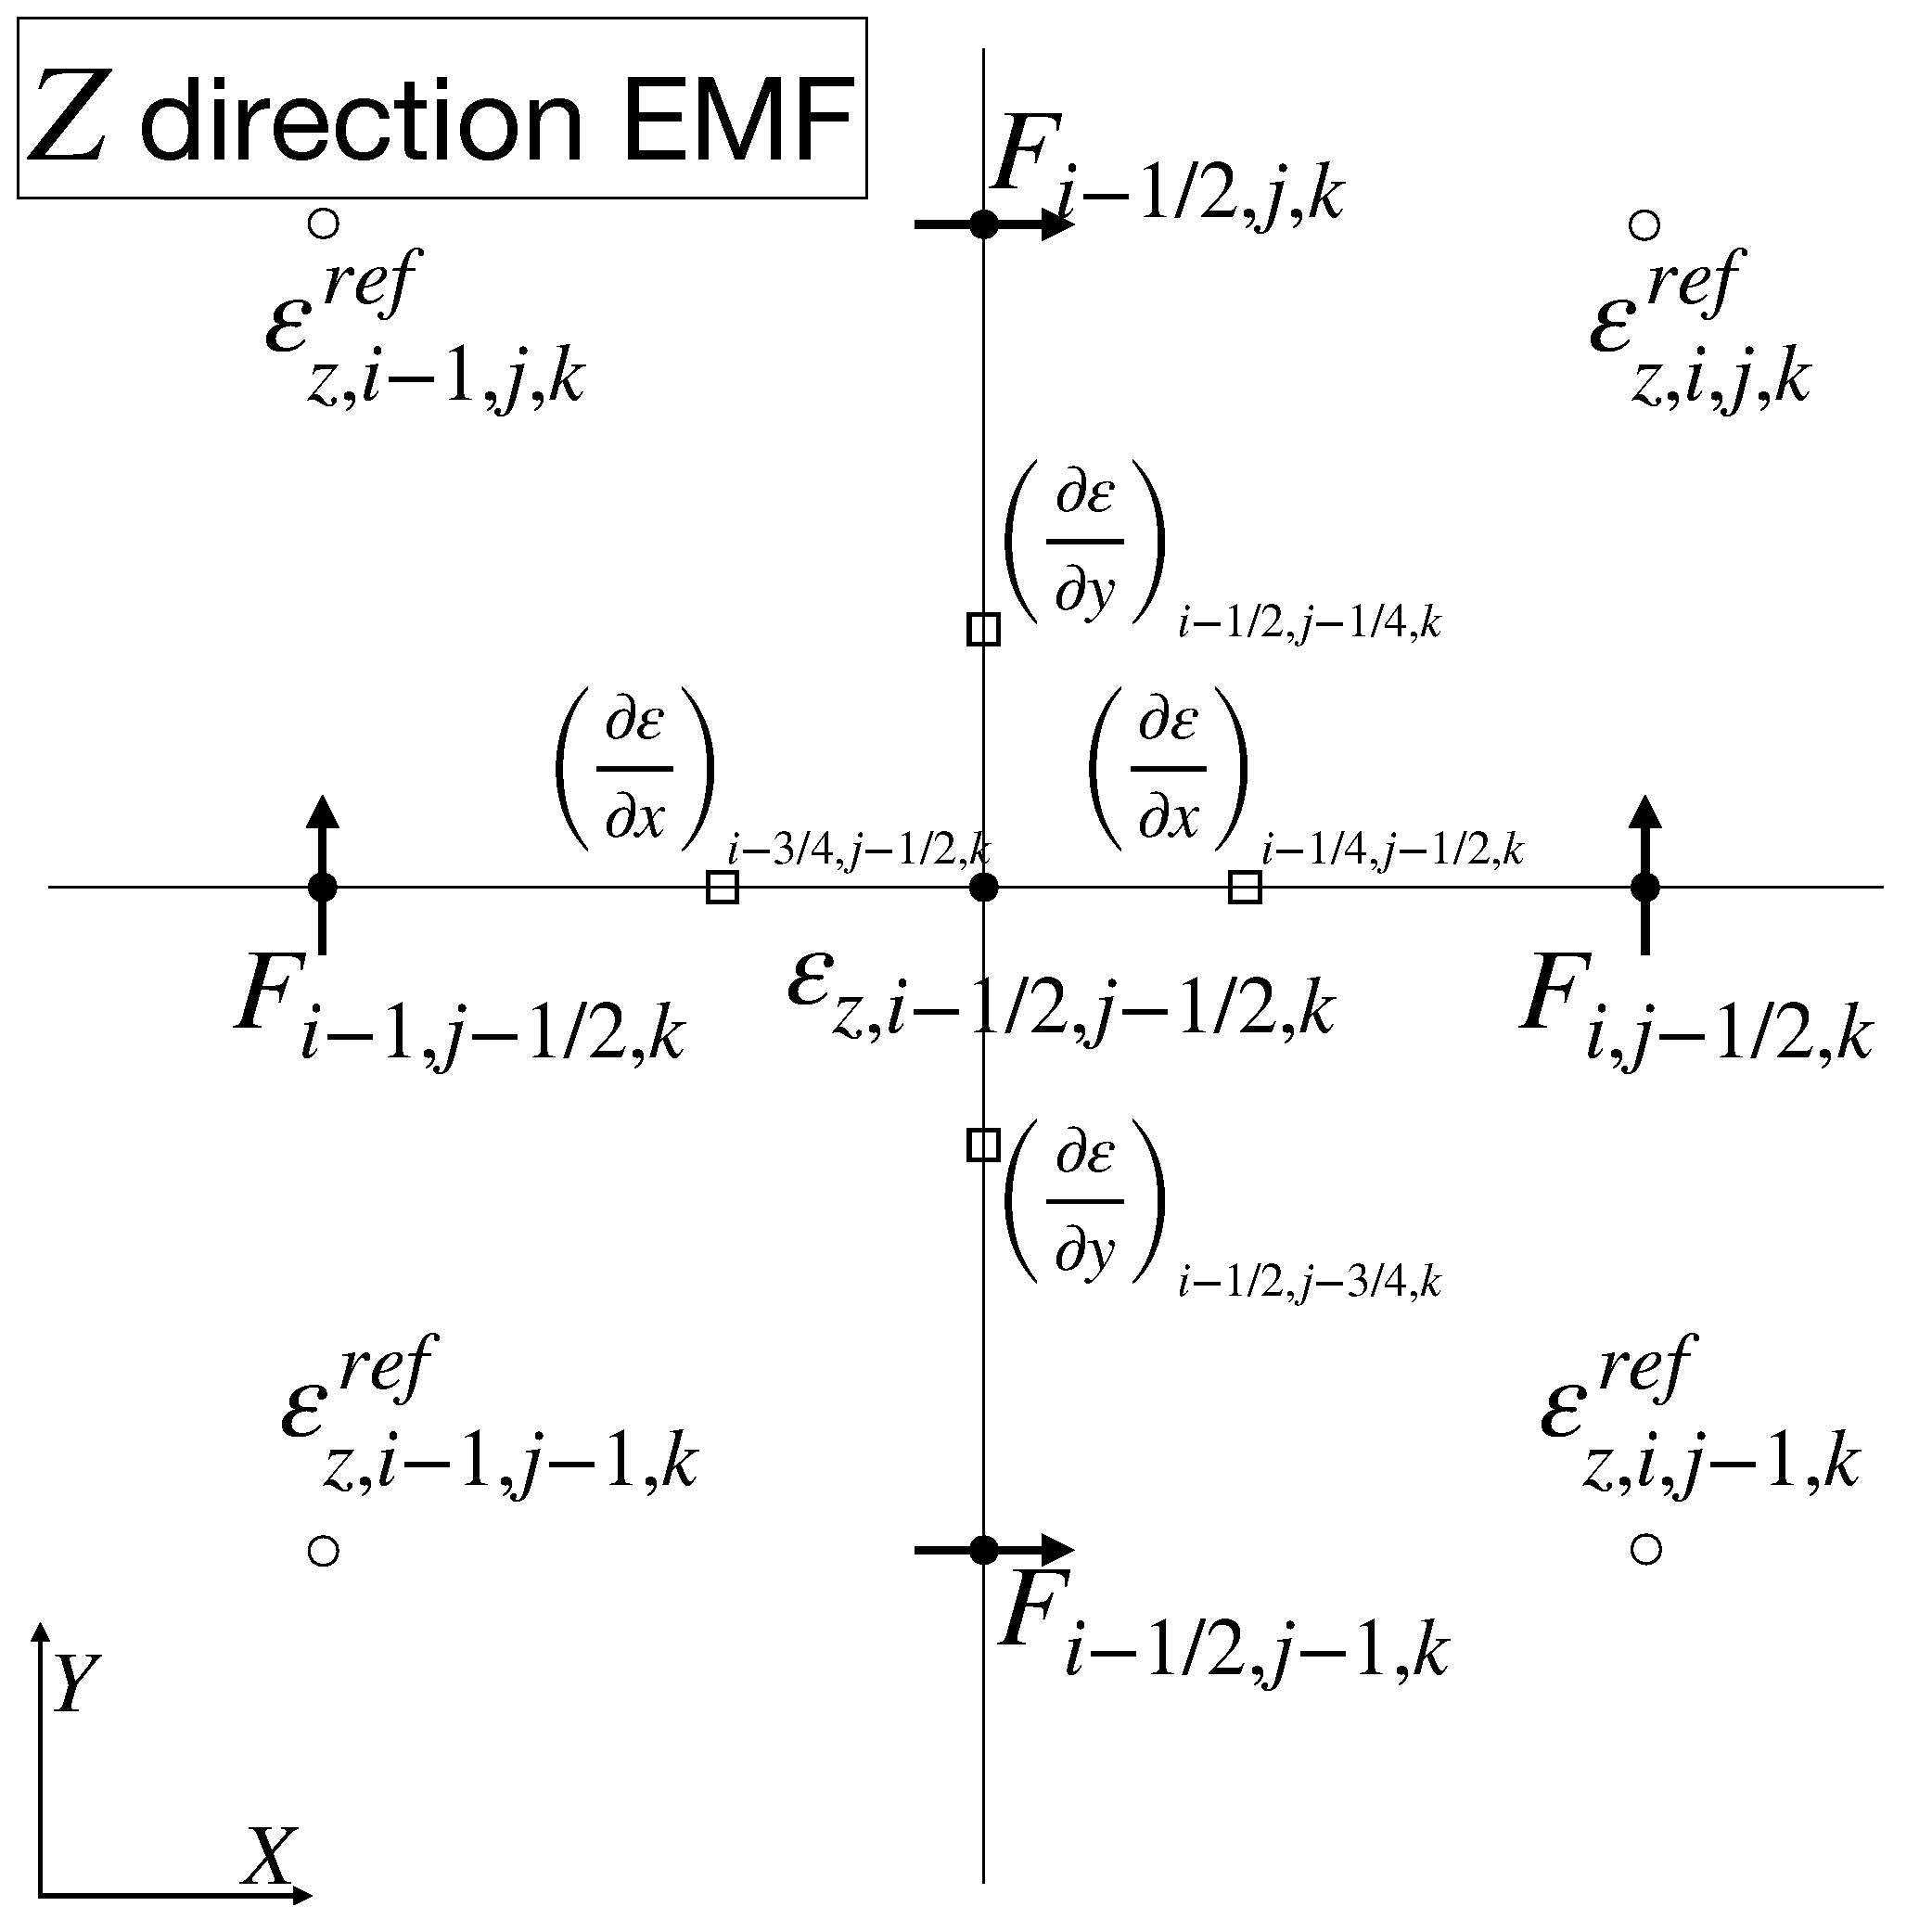
\includegraphics[width=0.5\linewidth]{CT-edge-field-figures-Z.pdf}
    \caption{2D slices in all three planes showing the location of the fluxes, edge electric fields, and derivatives. Based on Figure 5 of \cite{stone_athena_2008}.}
    \label{fig:emf-graph}
\end{figure}

\subsubsection{Step 5. Perform the Half Time-step Update}
\label{vlct:half-dt-update}

We first update the density, momenta, and energy, but not the magnetic fields, using the standard conservative update equation and the first-order fluxes from Step 3:

\begin{equation}
    \begin{aligned}
        \boldsymbol{U}^{n+1/2}_{i,j,k} = \boldsymbol{U}^{n}_{i,j,k}
        - \frac{\Delta t}{\Delta x} \left( \boldsymbol{F}^n_{x,i+1/2,j,k} - \boldsymbol{F}^n_{x,i-1/2,j,k} \right) \\
        - \frac{\Delta t}{\Delta y} \left( \boldsymbol{F}^n_{y,i+1/2,j,k} - \boldsymbol{F}^n_{y,i-1/2,j,k} \right) \\
        - \frac{\Delta t}{\Delta z} \left( \boldsymbol{F}^n_{z,i+1/2,j,k} - \boldsymbol{F}^n_{z,i-1/2,j,k} \right).
    \end{aligned}
\end{equation}

We then update the magnetic field using the electric fields computed in Step 4:

\begin{equation}
    \begin{aligned}
        B^{n+1/2}_{x,i-1/2,j,k} = B^{n}_{x,i-1/2,j,k}
        + \frac{\Delta t}{\Delta z} \left( \mathcal{E}^n_{y,i-1/2,j,k+1/2} - \mathcal{E}^n_{y,i-1/2,j,k-1/2} \right) \\
        - \frac{\Delta t}{\Delta y} \left( \mathcal{E}^n_{z,i-1/2,j+1/2,k} - \mathcal{E}^n_{z,i-1/2,j-1/2,k} \right)
    \end{aligned}
\end{equation}

\begin{equation}
    \begin{aligned}
        B^{n+1/2}_{y,i,j-1/2,k} = B^{n}_{y,i,j-1/2,k}
        + \frac{\Delta t}{\Delta x} \left( \mathcal{E}^n_{z,i+1/2,j-1/2,k} - \mathcal{E}^n_{z,i-1/2,j-1/2,k} \right) \\
        - \frac{\Delta t}{\Delta z} \left( \mathcal{E}^n_{x,i,j-1/2,k+1/2} - \mathcal{E}^n_{x,i,j-1/2,k-1/2} \right)
    \end{aligned}
\end{equation}

\begin{equation}
    \begin{aligned}
        B^{n+1/2}_{z,i,j,k-1/2} = B^{n}_{z,i-1/2,j,k}
        + \frac{\Delta t}{\Delta y} \left( \mathcal{E}^n_{x,i,j+1/2,k-1/2} - \mathcal{E}^n_{x,i,j-1/2,k-1/2} \right) \\
        - \frac{\Delta t}{\Delta x} \left( \mathcal{E}^n_{y,i+1/2,j,k-1/2} - \mathcal{E}^n_{y,i-1/2,j,k-1/2} \right).
    \end{aligned}
\end{equation}

\subsubsection{Step 6. Half Time-step Second Order Reconstruction}
\label{vlct:higher-order-reconstruction}

Step 5 results in first order time-averaged values for the cell-centered conserved variables and face-centered magnetic fields. To make the integration second-order in time, we need to perform a ``corrector" step. First, we perform a higher order interface reconstruction. The method shown here is for Piecewise Linear Method (PLM), reconstruction. Cholla currently implements piecewise constant, piecewise linear, and piecewise parabolic reconstruction, with limiting in the characteristic variables, for MHD. The piecewise parabolic method that Cholla utilizes is discussed in detail in \cite{felker_2018}. Using the third order piecewise parabolic method for spatial reconstruction does typically give slightly more accurate results at a given resolution compared to PLM, but since the method is formally second order it does not improve the overall order of convergence. Note that at a given face only the transverse components of the electric field need to be reconstructed. The longitudinal component is already given at the face.

The steps of the PLM update are:
\begin{enumerate}
    \item Compute the primitive variables from the conserved variables.

    \item Compute the left, right, centered, and Van Leer differences in the primitive variables
    \begin{align}
        \delta \boldsymbol{W}_{L,i} &= \boldsymbol{W_{i}} - \boldsymbol{W_{i-1}} \\
        \delta \boldsymbol{W}_{R,i} &= \boldsymbol{W_{i+1}} - \boldsymbol{W_{i}} \\
        \delta \boldsymbol{W}_{C,i} &= \frac{\boldsymbol{W_{i+1}} - \boldsymbol{W_{i-1}}}{2} \\
        \delta \boldsymbol{W}_{VL,i} &=
        \begin{cases}
            \frac{2 \boldsymbol{W}_{L,i} \boldsymbol{W}_{R,i}}{\boldsymbol{W}_{L,i} +\boldsymbol{W}_{R,i}} ,& \text{if } \boldsymbol{W}_{L,i} \boldsymbol{W}_{R,i} > 0\\
            0,              & \text{otherwise}
        \end{cases}
    \end{align}

    \item Project the slopes into the characteristic variables, $\boldsymbol{a}$, using the eigenvectors listed in the appendix of \cite{stone_athena_2008}. Note that to maintain mathematical consistency we use the eigenvectors of the $\boldsymbol{w_{i}}$ cell for all four slopes and the later projection back to primitive variables.
    \item Apply monotonicity constraints to the characteristic differences to ensure that the reconstruction is total variation diminishing (TVD). We use the following limiter, given in \cite{leveque2002finite}:
    \begin{equation}
        \label{eqn:limiter}
        \delta \boldsymbol{a}_{m,i} =
        \begin{cases}
             \text{sgn}(\boldsymbol{a}_{C,i})\min(2\abs{\boldsymbol{a}_{L,i}},2\abs{\boldsymbol{a}_{R,i}},\abs{\boldsymbol{a}_{C,i}},\abs{\boldsymbol{a}_{VL,i}}),& \text{if } \boldsymbol{a}_{L,i} \boldsymbol{a}_{R,i} > 0\\
            0,              & \text{otherwise}
        \end{cases}
    \end{equation}
    \item Project the limited characteristic slopes, $\delta \boldsymbol{a}_{m}$, back into the primitive variables, $\delta \boldsymbol{W}_{m}$, using the eigenvectors.
    \item Compute the interface states $\boldsymbol{W}_{L, i+1/2}$ and $\boldsymbol{W}_{R, i-1/2}$:
\end{enumerate}

    \begin{equation}
        \begin{aligned}
            \boldsymbol{W}_{L, i+1/2} = \boldsymbol{W}_{i} + \frac{\delta \boldsymbol{W}_{m, i}}{2} \\
            \boldsymbol{W}_{R, i-1/2} = \boldsymbol{W}_{i} - \frac{\delta \boldsymbol{W}_{m, i}}{2} \\
        \end{aligned}
    \end{equation}

    \noindent where $ \boldsymbol{W}_{L/R, i\pm1/2} $ is the state on the left or right side
    of the cell and $ \delta \boldsymbol{W}_{m, i} $ is the monotonically limited
    primitive slope. Limiting can be done in the primitive variables by skipping steps 3 and 5 and replacing the characteristic slopes in Equation \ref{eqn:limiter} with their primitive counterparts.

\subsubsection{Step 7. Second Riemann Solve}
\label{vlct:2nd-riemann-solve}

Solve the Riemann problem for each interface again using the higher order interface states computed in step 6.

\subsubsection{Step 8. Compute the Constrained Transport Electric Fields}
\label{vlct:2nd-emf}

Repeat step 3, but using the fluxes from the second Riemann solve and the half time step MHD variables computed in Step 5.

\subsubsection{Step 9. Perform the Full Time-step Update}
\label{vlct:full-dt-update}

Update the cell-centered hydro variables from $t = n$ to $t = n + \Delta t$ using the conserved update equation and the second order fluxes computed in Step 7:

\begin{equation}
    \begin{aligned}
        \boldsymbol{U}^{n+1}_{i,j,k} = \boldsymbol{U}^{n}_{i,j,k}
        &- \frac{\Delta t}{\Delta x} \left( \boldsymbol{F}^{n+1/2}_{x,i+1/2,j,k} - \boldsymbol{F}^{n+1/2}_{x,i-1/2,j,k} \right) \\
        &- \frac{\Delta t}{\Delta y} \left( \boldsymbol{F}^{n+1/2}_{y,i+1/2,j,k} - \boldsymbol{F}^{n+1/2}_{y,i-1/2,j,k} \right) \\
        &- \frac{\Delta t}{\Delta z} \left( \boldsymbol{F}^{n+1/2}_{z,i+1/2,j,k} - \boldsymbol{F}^{n+1/2}_{z,i-1/2,j,k} \right).
    \end{aligned}
\end{equation}

Update the face-centered magnetic field using the electric fields calculated in Step 8:

\begin{equation}
    \begin{aligned}
        B^{n+1}_{x,i-1/2,j,k} = B^{n}_{x,i-1/2,j,k}
        + \frac{\Delta t}{\Delta z} \left( \mathcal{E}^{n+1/2}_{y,i-1/2,j,k+1/2} - \mathcal{E}^{n+1/2}_{y,i-1/2,j,k-1/2} \right) \\
        - \frac{\Delta t}{\Delta y} \left( \mathcal{E}^{n+1/2}_{z,i-1/2,j+1/2,k} - \mathcal{E}^{n+1/2}_{z,i-1/2,j-1/2,k} \right)
    \end{aligned}
\end{equation}

\begin{equation}
    \begin{aligned}
        B^{n+1}_{y,i,j-1/2,k} = B^{n}_{y,i,j-1/2,k}
        + \frac{\Delta t}{\Delta x} \left( \mathcal{E}^{n+1/2}_{z,i+1/2,j-1/2,k} - \mathcal{E}^{n+1/2}_{z,i-1/2,j-1/2,k} \right) \\
        - \frac{\Delta t}{\Delta z} \left( \mathcal{E}^{n+1/2}_{x,i,j-1/2,k+1/2} - \mathcal{E}^{n+1/2}_{x,i,j-1/2,k-1/2} \right)
    \end{aligned}
\end{equation}

\begin{equation}
    \begin{aligned}
        B^{n+1}_{z,i-1/2,j,k} = B^{n}_{z,i-1/2,j,k}
        + \frac{\Delta t}{\Delta y} \left( \mathcal{E}^{n+1/2}_{x,i,j+1/2,k-1/2} - \mathcal{E}^{n+1/2}_{x,i,j-1/2,k-1/2} \right) \\
        - \frac{\Delta t}{\Delta x} \left( \mathcal{E}^{n+1/2}_{y,i+1/2,j,k-1/2} - \mathcal{E}^{n+1/2}_{y,i-1/2,j,k-1/2} \right).
    \end{aligned}
\end{equation}

\subsubsection{Step 10. Increment the Time by \texorpdfstring{$\Delta t$}{dt}}
\label{vlct:increment-time}

Increment the time by $\Delta t$. Additional physics modules are added in an operator-split fashion after this point (chemistry, radiation transport, etc.), after which all MPI communication is done to exchange the ghost/halo cells that surround each MPI rank's subdomain.

\subsection{Implementation on GPUs}
\label{sec:gpu-vs-cpu}

While the implementation of MHD on GPUs is similar to the implementation on CPUs there are some crucial differences, especially regarding data handling and movement. Compared to CPUs, GPUs have high memory bandwidth and extremely high FLOPS but limited memory capacity and limited functionality due to their fundamentally SIMD (Single Instruction Multiple Data) nature. Also, while GPU memory bandwidth is higher on the whole, due to their parallel nature GPUs can request many more values from memory at once, meaning codes are often still limited by memory bandwidth.

This leads to some implementation choices that may seem counter-intuitive. For example, while an optimized CPU-based code may compute the cell-centered magnetic fields once and then save them to memory, Cholla recomputes them in each function call where they are required. Similarly, Cholla does not store the primitive variables, only the conserved ones, and recomputes the primitive variables as needed. This approach reduces global memory usage by not storing an entire second grid. It also generally reduces memory bandwidth requirements, since often both the conserved and primitive variables are needed within a function, but only one set needs to be loaded.

Another major challenge in GPU computing is CPU-to-GPU bandwidth. While many systems have extremely fast GPU-to-GPU communications on-node, off-node data exchanges require data to be transported across a PCIe bus (in most cases), which can be a major performance bottleneck. This problem has been exacerbated in recent years, as nodes have become increasingly GPU-heavy and GPUs have reached higher peak performance, but bus speeds have only increased by a factor of a few.

To address this problem, Cholla now keeps as much data as possible in the GPU memory instead of moving it to and from main system memory, in contrast with previous versions of the code. Although it has always been a GPU-native code, historically Cholla used an extreme version of the ``offload" model of GPU programming, keeping the ``primary" data (like conserved variable arrays) in CPU memory, and copying that data the GPU to carry out computations before copying it back each time step. Although this approach originally had the advantage of allowing larger grid sizes to be computed on a single GPU, as GPUs have gotten dramatically faster and their memory capacity has increased over the last decade, these full-grid copies between CPU and GPU memory would now dominate the simulation run time. In addition, some new supercomputers, such as \textit{Frontier}, have GPUs that are directly connected to the network, so direct off-node GPU-to-GPU MPI communication is now possible. Between these two factors it is much more efficient to store all the simulation data on the GPU, and only move it back to the CPU for i/o operations. In the new version of Cholla described in this work, all computations are carried out on the GPU, and  MPI communication proceeds directly from GPU memory buffers. The only functions that remain on the CPU are the setting of the initial conditions, which only occurs once, and reading and writing output files.\footnote{At the time of writing, the HDF5 library does not support writing files directly from GPU memory.}

\subsubsection{GPU reductions}

There are several places in Cholla where a grid wide reduction must be performed. The primary example is the calculation of the time step, which requires finding the minimum crossing time in the full simulation grid. While CPU and MPI based reductions are relatively simple to implement, often through library calls, the inherently parallel nature of the GPU programming model makes GPU based reductions somewhat more complex. For GPU reductions in Cholla, we use a method similar to that described by NVIDIA\footnote{https://developer.nvidia.com/blog/faster-parallel-reductions-kepler/} which describe the challenges of a GPU reduction well. This reduction method uses atomics for the final level of reduction. At the time of writing, CUDA does not support floating point \texttt{atomicMax}. To work around this we have adopted a method from the RAPIDS cuML library\footnote{https://github.com/rapidsai/cuml/blob/dc14361ba11c41f7a4e1e6a3625bbadd0f52daf7/cpp/src\_prims/stats/minmax.cuh} which, with some encoding, uses the integral \texttt{atomicMax}. Overall this method is slightly faster than Cholla's previous hybrid GPU+CPU reduction for the number of elements we typically encounter. Primarily though, it is much simpler to use and performs dramatically better as the number of elements increases.

\section{MHD Tests}
\label{sec:mhd-tests}

\subsection{Linear Wave Convergence}
\label{sec:lwc}

The propagation of the four MHD linear waves provide an excellent quantitative measure of the accuracy of computation methods \citep{stone_2009}. The tests use a domain of $1.0\times1.0\times1.0$ and a resolution of $N\times16\times16$ where $N$ goes from 16 to 512 in powers of 2. The equation of the wave is

\begin{equation}
    q = \overline{q} + A R_w \sin{\frac{2\pi x}{\lambda}}
\end{equation}

where $q$ is the conserved variable, $\overline{q}$ is the mean background state, $A=10^{-6}$ is the amplitude of the wave, $R_w$ is the right eigenvector in conserved variables for the wave mode $w$, $x$ is the position, and $\lambda=1$ is the wavelength of the wave. The adiabatic index $\gamma$ is $5/3$ and the background state is: 
$\overline{\rho}=1.0$,
$\overline{v_x}=\overline{v_y}=\overline{v_z}=0$ (except for the contact wave where $\overline{v_x} = 1$),
$\overline{P}=1/\gamma$,
$\overline{B_x}=1$,
$\overline{B_y}=1.5$,
$\overline{B_z}=0$ 
and the right eigenvectors for this state are given in Appendix A of \cite{gardiner_unsplit_2008}. 

The wave is propagated for one period and then the error between the initial and final state is the L2 norm of the L1 error vector. First we compute the L1 norm of the absolute difference for each conserved variable between the initial and final state

\begin{equation}
    \delta q_s = \frac{1}{n_x n_y n_z} \sum_{i,j,k} \mid q^f_{i,j,k,s} - q^i_{i,j,k,s} \mid
\end{equation}

where $q_s$ is a specific conserved variable. We then compute the L2 norm of this vector of L1 norms

\begin{equation}
    \mid \mid \delta q \mid \mid = \sqrt{\sum_s \left( \delta q_s \right)^2}.
\end{equation}

These L2 errors are plotted in \autoref{fig:linear-wave-convergence} for both the PLM and PPM reconstructions. The results are comparable to the results in \cite{stone_2009} and demonstrate the expected second order convergence for this second order method. Using PPM does improve the accuracy of the method but maintains the second order convergence due to the second order nature of the integrator. These tests have been run in all three directions with the waves moving in the positive or negative directions and gotten identical results.

\begin{figure}[ht!]
    % \epsscale{0.5}
    \plotone{assets/3-mhd-tests/linear_convergence.pdf}
    \caption{Linear Wave Convergence of all four MHD waves using PLM and PPM reconstruction. \input{|python ../python/get_links.py 'linear_wave_convergence'}}
    \label{fig:linear-wave-convergence}
\end{figure}

\subsection{Circularly Polarized Alfv\'en Wave}
\label{sec:cpaw}

The circularly polarized Alfv\'en wave is a non-linear wave that allows one to test the codes accuracy in the non-linear regime with the quantitative benefits of a regular wave test. The tests use a domain of $3.0\times1.5\times1.5$ and a resolution of $2N\times N \times N$ where $N$ goes from 8 to 256 in powers of 2 and periodic boundary conditions. The wave is set to travel at an oblique angle the grid making this a fully 3D test.

In coordinate system aligned with the movement of the wave the initial conditions are 
$\rho = 1.0$,
$P = 0.1$,
$v_x = (0,-1)$ for traveling or standing waves respectively,
$v_y = A \sin{\frac{2\pi x}{\lambda}}$,
$v_z = A \cos{\frac{2\pi x}{\lambda}}$,
$B_x = 1.0$,
$B_y = A \sin{\frac{2\pi x}{\lambda}}$,
$B_z = A \cos{\frac{2\pi x}{\lambda}}$,
where the amplitude of the wave $A = 0.1$ and the wavelength $\lambda = 1.0$. These coordinates are then rotated with the following rotation

\begin{eqnarray}
    x\prime = x \cos\alpha\cos\beta - y \sin\beta - z \sin\alpha\cos\beta \nonumber \\
    y\prime = x \cos\alpha\sin\beta + y \cos\beta - z \sin\alpha\sin\beta \nonumber \\
    z\prime = x \sin\alpha + z \cos\alpha \nonumber
\end{eqnarray}

with $\sin\alpha = 2/3$ and $\sin\beta = 1/\sqrt{5}$. This ensures the domain is fully periodic through the boundaries and the wave can travel (or stand) indefinitely. The magnetic fields are initialized with the vector potential to ensure initial divergence is zero to round off. The waves are then run for a single period and the L2 norm of the L2 error vector is plotted in Figure \ref{fig:cpaw} using the same method as in Section \ref{sec:lwc}. It's especially interesting to note that the improvement in accuracy that PPM brought over PLM in the linear waves is absent in this non-linear test.

These Alfv\'en waves are subject to a parametric instability \citep{del_zanna_parametric_2001} which should not be present for these initial conditions. However, the truncation error will result in small variations in the magnetic pressure which will drive low amplitude compression waves \citep{stone_athena_2008}. 

\begin{figure}[ht!]
    % \epsscale{0.5}
    \plotone{assets/3-mhd-tests/cpaw_convergence.pdf}
    \caption{Circularly Polarized Alfv\'en Wave Convergence using PLM and PPM reconstruction. \input{|python ../python/get_links.py 'cpaw'}}
    \label{fig:cpaw}
\end{figure}

\subsection{Advecting Field Loop}
\label{sec:afl}

In this test we advect a tilted spherical current loop across the domain at an oblique angle to the grid. This test requires particularly accurate balancing of the non-zero components of the induction equation. It also has zero magnetic field outside the spherical current loop, as the current loops moves across the grid those cells that are no longer in the loop should return to zero; within round off. It is also a good test of the dissipation of the magnetic field as the magnetic pressure should remain constant.

The initial conditions for this test are most easily described using the vector potential. The background state is
$\rho = 1.0$,
$P = 1.0$,
$v_x = 1.0$,
$v_y = 1.0$,
$v_z = 2.0$,
$B_x = 0$,
$B_y = 0$,
$B_z = 0$.

In the central region the state is given by the following vector potential that we have chosen such that $A_x = 0$,
\begin{equation}
    A_y = A_z = 
    \begin{cases}
        A \left( R - r \right),& \text{for}\; r < R\\
        0,              & \text{otherwise}
    \end{cases}
\end{equation}

where $r$ is the Euclidean distance from the center of the domain. Note that since the vector potential is along the vertices of the cells $A_y$ and $A_z$ will never have the same value at the same position since they are not stored at identical positions. The test is conducted in a grid of $N\times N\times 2N$ cells for $N=(32, 64, 128, 256)$ with a domain of $1.0\times1.0\times2.0$ centered at zero and evolved for two periods; $t_{max} = 2.0$.

In Figure \ref{fig:afl} the mean of cell centered $B^2$ normalized to the initial value is plotted to show the convergence of the dissipation rate. The dissipation rate is comparable to those found in the literature \citep{stone_athena_2008} and improves at approximately first order. Figure \ref{fig:afl} also shows the maximum divergence in the domain as a function of time. Throughout the entire evolution it remains near round off and, after an initial rise, remains fairly constant. The zero magnetic field region outside of the current loop also remains near zero throughout the entire evolution of the problem.
 
\begin{figure}[ht!]
    % \epsscale{0.5}
    \plotone{assets/3-mhd-tests/afl.pdf}
    \caption{Evolution of tilted spherical magnetic field loop through two full periods. Mean of $B^2$ normalized to the initial value as a function of time (left) and the maximum divergence in the domain as a function of time (right). \input{|python ../python/get_links.py 'afl'}}
    \label{fig:afl}
\end{figure}

\subsection{MHD Riemann Problems}
\label{sec:riemann}

MHD Riemann problems are staple tests for new MHD codes and methods due to their mix of different flow types and extreme conditions. While there are a variety of different MHD Riemann problems in the literature \citep{brio_wu_1988, einfeldt_1991, ryu_jones_1995, dai_woodward_1998} we have chosen five that present a variety of challenging cases. 

The Riemann problem is defined as having a single state for half of the domain which suddenly switches to a different state on the other half of the domain. All of Riemann problems here have a domain of $1\times1\times1$ and resolution of $512\times16\times16$ and are run until the $t_{max}$ for that particular Riemann problem. All have been run in all three spatial directions with both possible orientations of the two states and achieved identical results. The details of each left and right state are in Table \ref{table:riemann} and the details of each Riemann problem are discussed in the captions of Figures \ref{fig:brio-and-wu}-\ref{fig:einfeldt}.

% Can add a * after "deluxetable" in begin and end to let it span 2 columns

%% The values (usually only l,r and c) in the last part of
%% \begin{deluxetable}{} command tell LaTeX how many columns
%% there are and how to align them.
\begin{deluxetable*}{lccccccccccccccccc}
    \label{table:riemann}
    
    %% Over-ride the default font size
    %% Use Default (12pt)
    
    %% Use \tablewidth{?pt} to over-ride the default table width.
    %% If you are unhappy with the default look at the end of the
    %% *.log file to see what the default was set at before adjusting
    %% this value.
    
    %% This is the title of the table.
    \tablecaption{Riemann Problem Initial Conditions}
    
    %% The \tablehead gives provides the column headers.  It
    %% is currently set up so that the column labels are on the
    %% top line and the units surrounded by ()s are in the 
    %% bottom line.  You may add more header information by writing
    %% another line between these lines. For each column that requries
    %% extra information be sure to include a \colhead{text} command
    %% and remember to end any extra lines with \\ and include the 
    %% correct number of &s.
    \tablehead{\colhead{Riemann Problem} & \colhead{$\gamma$} & \colhead{$t_{max}$} & \colhead{$B_x$} & 
    \colhead{$\rho_L$} & \colhead{$P_L$} & \colhead{$v_{x,L}$} & \colhead{$v_{y,L}$} & \colhead{$v_{z,L}$} & \colhead{$B_{y,L}$} & \colhead{$B_{z,L}$} & 
    \colhead{$\rho_R$} & \colhead{$P_R$} & \colhead{$v_{x,R}$} & \colhead{$v_{y,R}$} & \colhead{$v_{z,R}$} & \colhead{$B_{y,R}$} & \colhead{$B_{z,R}$}}
    
    %% All data must appear between the \startdata and \enddata commands
    \startdata
    % Riemann Problem      gamma           t_max  B_x                       rho_L  P_L    V_x,L  V_y,L  V_z,L B_y,L                       B_z,L                     rho_R   P_R    V_x,R   V_y,R V_z,R B_y,R                     B_z,R
    Brio \& Wu           & 2             & 0.1  & 0.75                    & 1    & 1    & 0    & 0    & 0   & 1                         & 0                       & 0.128 & 0.1  & 0     & 0   & 0   & -1                      & 0                       \\
    Dai \& Woodward      & $\frac{5}{3}$ & 0.2  & $\frac{2}{\sqrt{4\pi}}$ & 1.08 & 0.95 & 1.2  & 0.01 & 0.5 & $\frac{3.6}{\sqrt{4\pi}}$ & $\frac{2}{\sqrt{4\pi}}$ & 1     & 1    & 0     & 0   & 0   & $\frac{4}{\sqrt{4\pi}}$ & $\frac{2}{\sqrt{4\pi}}$ \\
    Ryu \& Jones 1a      & $\frac{5}{3}$ & 0.08 & $\frac{5}{\sqrt{4\pi}}$ & 1    & 20   & 10   & 0    & 0   & $\frac{5}{\sqrt{4\pi}}$   & 0                       & 1     & 1    & -10   & 0   & 0   & $\frac{5}{\sqrt{4\pi}}$ & 0                       \\
    Ryu \& Jones 4d      & $\frac{5}{3}$ & 0.16 & 0.7                     & 1    & 1    & 0    & 0    & 0   & 0                         & 0                       & 0.3   & 0.2  & 0     & 0   & 1   & 1                       & 0                       \\
    Einfeldt Rarefaction & 1.4           & 0.16 & 0                       & 1    & 0.45 & -2   & 0    & 0   & 0.5                       & 0                       & 1     & 0.45 & 2     & 0   & 0   & 0.5                     & 0                       \\
    \enddata
    
    %% Include any \tablenotetext{key}{text}, \tablerefs{ref list},
    %% or \tablecomments{text} between the \enddata and 
    %% \end{deluxetable} commands
    
    %% General table comment marker
    \tablecomments{The $L/R$ subscripts indicate that it is the left/right state. $B_x$ is always the same in both states.}
    
\end{deluxetable*}

\begin{figure}[ht!]
    % \epsscale{0.5}
    \plotone{assets/3-mhd-tests/b&w.pdf}
    \caption{Brio \& Wu Shock Tube solution. This is essentially the Sod shock tube with a magnetic field. However, this shock tube is an excellent stress test for the PPM reconstruction as PPM methods tend to create large oscillations in the solution due to the slowly moving shocks. To minimize these oscillations we implemented a new PPM reconstruction algorithm based on \cite{felker_2020} which reduced the oscillations to a reasonable level. No oscillation is present when using PLM reconstruction.
    \input{|python ../python/get_links.py 'b&w'}}
    \label{fig:brio-and-wu}
\end{figure}

\begin{figure}[ht!]
    % \epsscale{0.5}
    \plotone{assets/3-mhd-tests/d&w.pdf}
    \caption{Dai \& Woodward Shock Tube (also called Ryu \& Jones 2a) solution. This shock tube produces all seven possible MHD waves: from left to right a fast shock, Alfvén wave, slow shock, contact discontinuity, slow shock, Alfvén wave, and fast shock. This makes it an excellent laboratory for checking that the full spread of mave modes are well resolved
    \input{|python ../python/get_links.py 'd&w'}}
    \label{fig:dai-and-woodward}
\end{figure}

\begin{figure}[ht!]
    % \epsscale{0.5}
    \plotone{assets/3-mhd-tests/rj1a.pdf}
    \caption{Ryu \& Jones 1a Shock Tube solution. This shock tube has a fairly simple wave structure without any spikes which makes it easy to use for debugging purposes and a good test for over/undershoot of the solution near discontinuities.
    \input{|python ../python/get_links.py 'rj1a'}}
    \label{fig:rj-1a}
\end{figure}

\begin{figure}[ht!]
    % \epsscale{0.5}
    \plotone{assets/3-mhd-tests/rj4d.pdf}
    \caption{Ryu \& Jones 4d Shock Tube solution. This test features a switch-on slow shock. Switch-on waves increase the strength of the transverse magnetic field while reducing the thermal pressure to maintain energy conservation. This is a simplified example of a potential type of magnetic field amplification in galaxies and as such it is important that we replicate it accurately. A "switch-off" wave does the inverse.
    \input{|python ../python/get_links.py 'rj4d'}}
    \label{fig:rj-4d}
\end{figure}

\begin{figure}[ht!]
    % \epsscale{0.5}
    \plotone{assets/3-mhd-tests/einfeldt.pdf}
    \caption{MHD Einfeldt Strong Rarefaction solution. This Riemann problem simulates a strong outflow and central vacuum state. These diverging fluids lead to an extremely strong and fast rarefaction where the energy is dominated by kinetic energy and as such can often reveal issues in code accuracy since it can lead to nonphysical states with negative density or negative internal energy. High values of the outflow velocity ($V_{out}\ge3$) can lead to spurious oscillations so $V_{out} = 2$ was chosen\citep{charm_2011}.
    \input{|python ../python/get_links.py 'einfeldt'}}
    \label{fig:einfeldt}
\end{figure}

\subsection{MHD Blast Wave in a Strongly Magnetized Medium}
\label{sec:mhd-blast}

Blast waves in different forms are staple tests for hydrodynamics and MHD codes. They combine strong shocked flows, smooth flows, and, in MHD, strong magnetic fields. The results are qualitative rather than quantitative but thoroughly test the robustness of the algorithm and act act as an excellent regression test for our automated testing (see Section \ref{sec:testing}). In this test $\beta = 0.2$, like \cite{stone_2009} we note instability if $\beta$ is decreased by a factor of 10. This issue could possibly be resolved by integrating the internal energy separate from the total energy using the dual energy formalism in Cholla.

The background state is
$\rho = 1.0$,
$P = 0.1$,
$v_x = 0.0$,
$v_y = 0.0$,
$v_z = 0.0$,
$B_x = 1/\sqrt{2}$,
$B_y = 1/\sqrt{2}$,
$B_z = 0.0$,
and the over pressure region is a central sphere of size $R = 0.1$ which has $P=10.0$.

The test was then run with a domain of $1\times1.5\times1$ and resolution of $200\times300\times200$ until $t = 0.2$. Figure \ref{fig:blast} shows contours in the density and magnetic energy in an $x-y$ slice through the center of the domain. The contours are smooth and symmetric and show clear elongation of the blast wave rarefaction parallel to the magnetic field. The blast wave propagates slowly parallel to the magnetic field but much more rapidly perpendicular to the magnetic field

\begin{figure}[ht!]
    % \epsscale{0.5}
    \plotone{assets/3-mhd-tests/mhd-blast.pdf}
    \caption{Contour plot of the MHD blast wave test at $t=0.2$. 30 evenly spaced contours are shown in an $x-y$ slice through the center of the domain. \input{|python ../python/get_links.py 'mhd-blast'}}
    \label{fig:blast}
\end{figure}

\subsection{Orszag-Tang Vortex}
\label{sec:otv}

The Orszag-Tang vortex is a standard 2D MHD test from (CITE Orszag \& Tang (1979)). While it does not provide a quantitative measure of accuracy like the linear wave tests or a test of the robustness of the method like the MHD blast wave it does have a very complex flow that is sensitive to changes in the integrator; making it ideal for regression testing.

The test was conducted with a periodic domain of $1\times1\times1$ and resolution of $192\times192\times192$ until $t = 0.5$ with the following initial conditions: 
$\rho = 25 / \left( 36 \pi \right)$,
$P    =  5 / \left( 12 \pi \right)$,
$v_x  = \sin 2\pi y$,
$v_y  = -\sin 2\pi x$,
$v_z  = 0.0$,
$A_x  = 0.0$,
$A_y  = 0.0$,
$A_z  = \left( B_0/4\pi \right) \left( \cos{4\pi x} + 2 \cos{2\pi y} \right)$, with $B_0 = 1/sqrt{4\pi}$.

The results, plotted in Figure \ref{fig:otv}, can be compared directly to Figure 22 in \cite{stone_athena_2008} as a qualitative check for correctness of the flow structure.

\begin{figure}[ht!]
    % \epsscale{0.5}
    \plotone{assets/3-mhd-tests/orszag-tang-vortex.pdf}
    \caption{Contour plot of the Orszag-Tang Vortex at $t=0.5$. Thirty evenly spaced contours are shown for each plot in an $x-y$ slice through the center of the domain.  \input{|python ../python/get_links.py 'otv'}}
    \label{fig:otv}
\end{figure}

\section{MHD Performance Tests}
\label{sec:mhd-perf-tests}

The performance and weak scaling of MHD in Cholla is critical given the scale of the machines that Cholla is designed to run on. 


% Performance on different hardware: CRC V100+PPC, CRC A100+x86, Summit, Frontier, Grace Hopper?

\subsection{Weak Scaling}

\begin{figure}[ht!]
    % \epsscale{0.5}
    \plotone{assets/3-mhd-tests/scaling_tests_ms_per_gpu.pdf}
    \caption{CAPTION  \input{|python ../python/get_links.py 'scaling_plot'}}
    \label{fig:scaling-ms-per-gpu}
\end{figure}


\subsection{Cell Updates Per Second Per GPU}

\begin{figure}[ht!]
    % \epsscale{0.5}
    \plotone{assets/3-mhd-tests/scaling_tests_cells_per_second.pdf}
    \caption{CAPTION  \input{|python ../python/get_links.py 'scaling_plot'}}
    \label{fig:scaling-cells-per-second}
\end{figure}


\section{Automated Testing \& Continuous Integration}
\label{sec:testing}

As Cholla has continued to grow in complexity, and with the continued addition of large new physics modules like MHD that require changes to much of the code base, the need for a more robust, automated testing system has become increasingly apparent. Several challenges exist in implementing such a system for Cholla - not only must the testing system accommodate GPU hardware, but it must also work on large parallel systems like \textit{Frontier}. We have addressed this need in three primary steps: 1) Choosing a testing framework for unit tests, 2) Writing the software tools needed to extend that testing framework for Cholla's needs, and 3) adding automated testing as part of a continuous integration (CI) pipeline that runs whenever anyone submits a pull request to the Cholla GitHub repository. This Section describes the implementation of our automated testing and continuous integration framework.

Taken together, the ability to add tests for any part of the code and their automated running on every pull request has meant that new features are faster and easier to add to Cholla with confidence. Any errors or changes that break older code will likely be quickly caught by the tests before they ever make it into Cholla and have been successful in doing so.

\subsection{Unit Testing Framework}
\label{sec:testing-framework}

There are three main kinds of tests that we need for scientific code bases: unit tests, integration tests, and system tests (also called ``end-to-end" tests). Unit tests check that a single ``unit" of code, a single function, class method, data structure, etc. Integration tests check how units of code operate together. For example, a test of the HLLD solver is an integration test because the solver internally calls many different functions and uses multiple different data structures. System tests check the entire code base, often with a simple test problem like a Riemann problem or linear wave, and verify that the entire program produces the correct output.

GoogleTest\footnote{https://github.com/google/googletest} was chosen for as the testing framework. We chose GoogleTest for the unit testing framework due to its large number of features, general popularity, and relative ease of use. Another primary requirement was a testing framework that supports death tests, tests that check if the internals of the test crash/segfault/etc. Since Cholla, like many HPC codes, handles errors by reporting those errors and then exiting, a testing framework that can handle code crashes without crashing the tests as well is critical. GoogleTest is available already built on most of the HPC systems that we utilized and, if it is not available, can be built as an optional part of the test running script.

\subsection{Extensions for Cholla}

Two primary extensions were required for fully testing Cholla: a robust method for comparing floating point numbers and a way to run system tests.

\subsubsection{Floating Point Comparisons}
\label{sec:fp-comparing}

In order to run either unit tests or system tests, the code must have a robust method for comparing floating point numbers for equality. Comparing floating point numbers for equality is a notoriously challenging\footnote{https://randomascii.wordpress.com/2012/02/25/comparing-floating-point-numbers-2012-edition/} and generally the exact comparison method that should be used varies by application. Absolute comparisons ($|a-b| < X$) work well for small numbers, but with larger numbers the difference between two successive floats can be much larger than a typical value for $X$ and therefore a different comparison method is required. We chose a hybrid method of both an absolute comparison and a Units in Last Place (ULP) comparison. A ULP comparison determines how many representable floating point numbers there are between any two floats. By default the hybrid method first performs an absolute check, $|a-b| < 10^{-14}$. This number was chosen as we found that typical differences in the Sod Shock Tube solution when comparing results with different hardware and compilers resulted in differences of $\sim5\times10^{-15}$. After the absolute check a ULP check is performed with a maximum allowed error of 4. If either check passes then the numbers are deemed to be ``equal". GoogleTest does provide utilities to compare floating point numbers but they only utilize the ULP check which often fails when checking small numbers for equality.

\subsubsection{System Tests}

GoogleTest provides most of the tools required to run unit and integration tests, but validating the results of an entire system test is much more complex. Running a system test requires launching the program to test with correct initial conditions, checking that the program did not crash, loading both the generated data to test and the fiducial data, then comparing those two data sets. In order to perform system tests with Cholla, we added a class that performs all of the required tasks, which include launching Cholla with any number of MPI ranks as well as comparing the results against fiducial data. To facilitate running on across a wide range of MPI ranks and on clusters with queue systems, the class is designed to allow system tests to be run in different modes: one can either launch Cholla and save the results, compare already existing test data to fiducial data, or do both. This enables the user to run Cholla on many thousands of ranks then later launch a separate job to make the actual comparison. We have found that on up to 10,000 ranks, with small simulation grids (typically $<64^3 cells$) per rank the latter comparison only takes a few minutes on a single CPU core. Most of the time however, both steps can be run within the same job, since large tests with many ranks are not required for most development work.

Two primary methods of comparison are used to determine the success of a system test. These are either a direct cell-by-cell comparison of the results for each field using the floating point comparison tools described above (Section \ref{sec:fp-comparing}), or a calculation of the L2 norm of the L1 error vector as described in Section  \ref{sec:lwc}. The cell-by-cell comparison is quite accurate, but can be fragile on some complex tests if a small number of cells have errors that are slightly larger than typical which and can lead to false failures when comparing results between systems or compilers. The L2 norm method is less fragile to small errors in a handful of cells, but is generally less sensitive so we only use it on the tests where it is required, namely the MHD blast wave (\autoref{sec:mhd-blast}) and advecting field loop (\autoref{sec:afl}). Both methods are used since the L2 norm method can give false passes when a large number of cells are slightly off as is common if the test has erroneous oscillations, the cell-by-cell comparison does an excellent job of catching those kinds of errors in is also a more stringent comparison method.
 
\subsection{Automated Testing}

To ensure that these tests are run regularly and all new code is tested we have made the existing tests as easy to run as possible, and we require that they are all are run automatically on each pull request. To facilitate this, Cholla's build directory includes a script which performs all required setup, installs GoogleTest (if requested), builds Cholla, and then runs all the tests. The script also includes a function that combines all of these into a single function call for ease of use, for example, if a user is running tests manually (say, prior to submitting a PR). 

Implementing automated testing is not always an easy task. Automated tests are an aspect of Continuous Integration (CI) is the practice of automating the addition of code changes and additions from a team of developers into a software project. Cholla is currently designed to run on CUDA or HIP capable GPUs, so GPU hardware is required in order to incorporate continuous integration (CI) -- something that few current CI services offer at a reasonable cost for academic users. Our solution to this issue was to use a mix of two different systems. When a pull request is submitted to the Cholla GitHub repository several jobs are launched: A GitHub Actions\footnote{https://github.com/features/actions} job to check code formatting, a GitHub actions matrix job to build all the HIP/AMD builds, and a Jenkins\footnote{https://www.jenkins.io} matrix job running on CRC hardware that runs the CUDA builds, tests, and static analyzers. Thus, every common configuration of Cholla is built with both CUDA and HIP on every pull request and the CUDA builds are also tested to ensure that no existing or new tests fail. 




\section{Summary}
\label{sec:summary}

In this work we have presented the MHD extension of Cholla, a massively parallel, GPU native, MHD code. MHD in Cholla uses the Van Leer plus Constrained Transport MHD integrator \citep{stone_2009}, the HLLD Riemann solver, and multiple reconstruction methods to model numerical solutions to the Eulerian ideal MHD equations on a static mesh.

Designing the MHD extension to run on GPUs required some significant changes to the implementation compared to a CPU code and elicited challenges working within the limits of GPUs. The entire grid must stay in GPU memory to minimize the amount of data being passed between the CPU and GPU. GPUs also require specific memory layouts and a greater focus on reducing memory usage, even at the cost of increased computation. As demonstrated in Section \ref{sec:mhd-perf-tests}, these optimizations, and the highly parallel nature of GPUs, makes MHD in Cholla extremely fast, over 150 million cell updates per GPU-second even when scaled up to 74,088 GPUs for a total of over 11 trillion cell updates per second. 

We also present a suite of canonical MHD tests, Section \ref{sec:mhd-tests}. These tests demonstrate the accuracy of the code in a variety of ways and that the code does an excellent job of maintaining the divergence free condition even in highly challenging settings. 

As the complexity of Cholla and the number of people contributing to the code grew it quickly became clear that a more structured testing methodology was needed, Section \ref{sec:testing-framework}. To this end we adopted the GoogleTest\footnote{https://github.com/google/googletest} unit testing framework. Paired with some custom testing tools this enabled us to easily write and run tests ranging from simple unit tests all the way to massively parallel system tests with ease. We then integrated these tests with GitHub Actions\footnote{https://github.com/features/actions} to run formatting, static analysis, and builds with various configuration along with Jenkins\footnote{https://www.jenkins.io} running on University of Pittsburgh's cluster to run the tests. This enables us to easily run the tests on ever single pull request and catch bugs before they ever make it into the codebase.

% Future work
In the future we expect to apply this code to a high resolution ($\approx 10,000^3$ cells) simulation of a Milky Way like galaxy to study the impact of magnetic fields on the galactic winds and the dynamics of the galactic dynamo.
\section{Acknowledgements}

\begin{enumerate}
    \item Evan (will be on paper, idk if she should be included here too)
    \item Alwin (might be on the paper depending on how much we talk about the stuff he's done)
    \item Helena (made some utils files, I/O routines for dust, spearheaded the naming and formatting stuff)
    \item Orlando
    \item Thank you to Seth Cook for his unwavering support and help with technical issues.
    \item Funding
    \item Compute time
\end{enumerate}

\appendix

\section{MHD Equation Glossary}
\label{sec:mhd-glossary}
\section{HLLD Summary}
\label{sec:hlld}

I have this written up \href{https://robertcaddy.com/posts/HLLD-Algorithm/}{here} but haven't decided if I'll include it. I really want to include the VL+CT stuff since it's not really well spelled out in the series of Athena papers but the HLLD paper is pretty clear, if a bit out of order for implementing.

\bibliography{bibliography.bib}

\end{document}